\documentclass{ctexart}
\usepackage{amsmath}
\usepackage{rotating}
\usepackage{xparse,tikz}
\usetikzlibrary{calc}
\usepackage[margin = 2cm]{geometry}
\usepackage{graphicx}
\usepackage{zhnumber}
\usepackage{float} 
\usepackage{booktabs}
\usepackage{subcaption}
\newcommand{\Zzero}{Z_0}

\NewDocumentCommand{\makecover}{}{
  \begin{titlepage}
  \begin{center}
  \vspace*{5cm}
  {\LARGE\bfseries 电磁场与电磁波}\par
  \vspace{1.5cm}
  {\Large\bfseries 微带传输线负载特性矢网测量}\par
  \vspace{1cm}
  {\large 实验报告}
  \end{center}
  \end{titlepage}
}

\NewDocumentCommand{\makecoveri}{}{
  \begin{center}
  \begin{minipage}[c][145pt][c]{\textwidth}
  \centering{\Large\bfseries 电磁场与电磁波}\par
  \vspace{1cm}
  {\large 微带传输线负载特性矢网测量}
  \end{minipage}
  \end{center}
}

\newcounter{makepart}
\setcounter{makepart}{1}
\NewDocumentCommand{\makepart}{+m}
{
  \vspace{1em}
  \begin{flushleft}
   \large\bfseries\zhnumber{\arabic{makepart}}、#1
  \end{flushleft} 
  \stepcounter{makepart}
}

\NewDocumentCommand{\zdx}{}
{
  \tikz[remember picture,overlay]{
    \coordinate (s) at ([shift={(1,-3)}]current page.north west);
    \coordinate (e) at ([shift={(1,3)}]current page.south west);
    \foreach \x in{0,0.15,...,9.2}
    {
      \fill[] ($(s)+(0,-\x)$) circle(1pt);
    }
    \foreach \x in{0,0.15,...,9.2}
    {
      \fill[] ($(e)+(0,\x)$) circle(1pt);
    }
    \node[text width=1em,align=center]at($(s)!0.5!(e)$){装\\[10pt]订\\[10pt]线};
  }
}

\pagestyle{empty}

\begin{document}
\makecover
\makecoveri
\zdx



\section{实验目的与任务}

\subsection{实验目的}

理解传输线的基本特性，掌握微带传输线的结构特点、工作方式及负载变化对反射特性的影响。熟悉矢量网络分析仪测量微波网络参数的基本方法，掌握反射测量、传输测量、校准、显示格式选择和光标读数等操作。通过微带传输线负载、微带耦合滤波器和天线的测量，把 Smith 圆图、复阻抗、反射系数、驻波比、插入损耗和相位等量与实际电路状态联系起来。

\subsection{实验内容与任务}

\begin{enumerate}
  \item 用矢量网络分析仪测量微带开路传输线模块的反射特性，并分别接入开路、短路、49.9 $\Omega$ 电阻、1 pF 电容和 3.3 nH 电感负载，分析不同负载下的输入阻抗、反射系数和驻波比。
  \item 用矢量网络分析仪测量微带耦合滤波器的传输特性，读取 S21 幅度、相位、3 dB 带宽、中心频率和插入损耗，并观察外界扰动对通带响应的影响。
  \item 用矢量网络分析仪测量天线的反射特性和驻波比，判断其在 1 GHz 至 3 GHz 频段内的主要匹配频点。
\end{enumerate}

\subsection{实验对象与仪器}

实验对象为工作频率约 2.5 GHz、特性阻抗约 50 $\Omega$ 的半波长微带传输线和微带平行耦合带通滤波器。微带基板参数为：相对介电常数 $\varepsilon_r=4.6$，介质厚度 $h=0.765\,\mathrm{mm}$，铜箔厚度约 $0.035\,\mathrm{mm}$，损耗正切约 0.015。主要仪器与附件包括 AV3656A 矢量网络分析仪、射频电缆、N-SMA 转接头、开短负载校准件、微带电路模块、贴片电阻/电容/电感及防静电镊子。

\section{实验原理}

\subsection{矢量网络分析仪测量量}

矢量网络分析仪并不是直接测量“电压表意义上的电压”，而是把被测网络看成由端口连接的微波网络，比较端口处入射波与出射波的幅度和相位。以二端口网络为例，有
\begin{equation}
  \begin{bmatrix}
    b_1 \\ b_2
  \end{bmatrix}
  =
  \begin{bmatrix}
    S_{11} & S_{12}\\
    S_{21} & S_{22}
  \end{bmatrix}
  \begin{bmatrix}
    a_1 \\ a_2
  \end{bmatrix},
\end{equation}
其中 $a_i$ 为第 $i$ 个端口的入射波，$b_i$ 为出射波。单端口反射测量时，本实验主要使用 $S_{11}=b_1/a_1$，它等价于端口参考面处的反射系数；滤波器传输测量时，主要使用 $S_{21}=b_2/a_1$，它反映信号从端口 1 传到端口 2 后的衰减和相位变化。

矢网测量必须强调参考面。仪器屏幕上的阻抗、反射系数和相位都属于校准参考面处的结果。若校准参考面停留在电缆端，而后面又接入 N-SMA 转接头、SMA 座、微带过渡和贴片元件压接结构，那么这些结构的电长度和不连续性都会进入测量结果。本实验后续对“端口等效阻抗”的表述，均指矢网参考面向被测微带结构看进去得到的等效量。

\subsection{传输线反射模型}

微带线在 2 GHz 以上已经不能简单看作低频导线。只要线长与波长可比，线上任一点的电压和电流都由入射波与反射波叠加形成。图 \ref{fig:ref-transmission-model} 给出了负载端传输线模型。

\begin{figure}[!htbp]
  \centering
  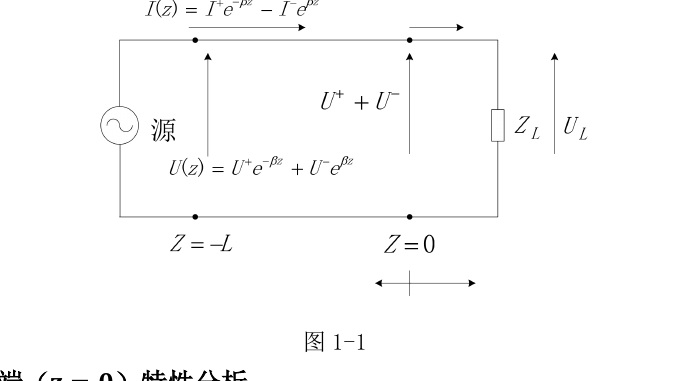
\includegraphics[width=0.68\textwidth]{figures/ref_transmission_model.png}
  \caption{传输线入射波与反射波模型}
  \label{fig:ref-transmission-model}
\end{figure}

设传输线特性阻抗为 $\Zzero$，传播常数为 $\gamma=\alpha+j\beta$。在损耗较小时可近似取 $\alpha\approx0$，线上电压可写成
\begin{equation}
  U(z)=U^+e^{-j\beta z}+U^-e^{j\beta z},
\end{equation}
电流可写成
\begin{equation}
  I(z)=\frac{U^+}{\Zzero}e^{-j\beta z}
      -\frac{U^-}{\Zzero}e^{j\beta z}.
\end{equation}
负载端反射系数定义为
\begin{equation}
  \Gamma_L=\frac{U^-}{U^+}.
\end{equation}
由负载端 $Z_L=U_L/I_L$ 可得
\begin{equation}
  \Gamma_L=\frac{Z_L-\Zzero}{Z_L+\Zzero},
  \label{eq:gamma-load}
\end{equation}
或写成归一化阻抗 $z_L=Z_L/\Zzero$ 的形式：
\begin{equation}
  z_L=\frac{1+\Gamma_L}{1-\Gamma_L}.
\end{equation}
因此，匹配负载 $Z_L=\Zzero$ 时 $\Gamma_L=0$；开路和短路时 $|\Gamma_L|=1$，只是相位分别对应 Smith 圆图右端和左端；电容、电感负载则在外圆附近分别落入容性和感性区域。

\subsection{输入阻抗变换与半波长微带线}

实际测量时仪器端口通常不在负载端，而是通过一段微带线看到负载。距负载 $l$ 处的输入阻抗为
\begin{equation}
  Z_\mathrm{in}=\Zzero
  \frac{Z_L+j\Zzero\tan(\beta l)}
       {\Zzero+jZ_L\tan(\beta l)}.
  \label{eq:zin}
\end{equation}
这个式子解释了一个很重要的现象：贴片电阻、电容、电感的标称值只是负载端局部元件值，矢网屏幕上的 $R+jX$ 是经过微带线变换后的输入阻抗。若 $l=\lambda/2$，则 $\tan(\beta l)=0$，理想无耗情况下有 $Z_\mathrm{in}=Z_L$；若频率偏离设计中心，$\beta l$ 不再正好等于 $\pi$，同一负载在 Smith 圆图上会沿等驻波比圆旋转。

本实验使用的微带传输线设计工作频率约为 2.5 GHz，特性阻抗约为 50 $\Omega$，线长约为导波半波长。由于微带线的电场一部分在介质板内、一部分在空气中，传播速度由有效介电常数决定，且开路端、连接器和压接元件会带来额外的端部效应。

\subsection{Smith 圆图判读}

Smith 圆图把复反射系数平面和归一化阻抗平面映射到同一个圆内，如图 \ref{fig:ref-smith-features} 所示。圆心为匹配点，右端为开路点，左端为短路点；水平实轴为纯电阻线，上半圆对应感性电抗，下半圆对应容性电抗；以圆心为圆心的圆对应等 $|\Gamma|$，也就是等驻波比圆。

\begin{figure}[!htbp]
  \centering
  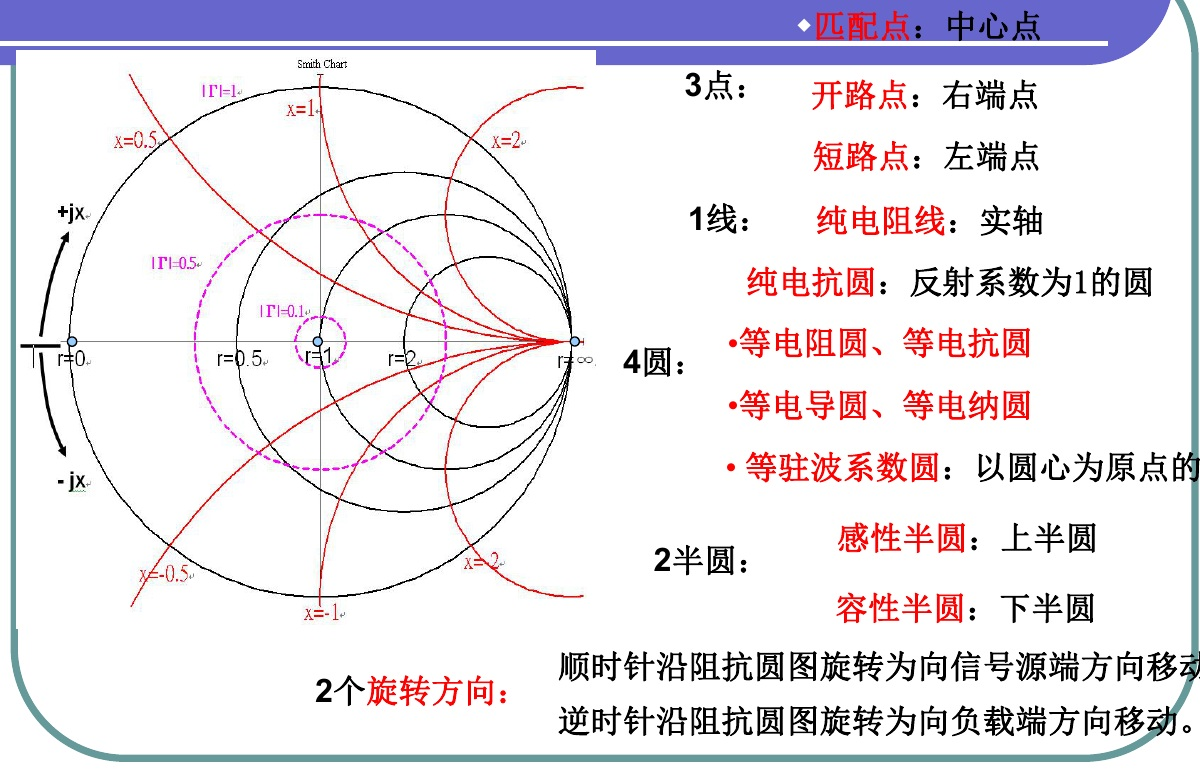
\includegraphics[width=0.58\textwidth]{figures/ref_smith_features.png}
  \caption{Smith 圆图主要特征与阻抗区域}
  \label{fig:ref-smith-features}
\end{figure}

读数时主要利用 Smith 圆图的两层信息。第一层是点的位置：越靠近圆心，匹配越好；越靠近外圆，反射越强。第二层是旋转方向：沿传输线向信号源移动时，阻抗点会在 Smith 圆图上旋转。因而短路负载并不一定始终显示在最左端，开路负载也不一定始终显示在最右端，实际位置取决于频率、微带线电长度和参考面。

反射系数模值可进一步换算为驻波比
\begin{equation}
  \mathrm{VSWR}=\frac{1+|\Gamma|}{1-|\Gamma|},
  \label{eq:vswr}
\end{equation}
回波损耗为
\begin{equation}
  RL=-20\log_{10}|\Gamma|.
  \label{eq:return-loss}
\end{equation}
驻波比越接近 1，端口匹配越好；回波损耗越大，反射越小。后续复阻抗换算均以 $\Zzero=50\,\Omega$ 为参考。

\subsection{平行耦合微带滤波器}

微带滤波器部分采用平行耦合线带通结构。其基本单元可以理解为半波长开路微带谐振器，多个谐振器通过相邻边缘场耦合形成带通响应。二端口测量时，滤波器连接在矢网两个端口之间，如图 \ref{fig:ref-filter-test} 所示。$S_{21}$ 的幅频曲线给出滤波器通带和阻带，$S_{21}$ 相位曲线反映信号通过滤波器的相移。常用性能指标包括中心频率 $f_0$、3 dB 带宽 $\Delta f=f_2-f_1$、品质因数
\begin{equation}
  Q=\frac{f_0}{\Delta f},
  \label{eq:q}
\end{equation}
插入损耗、带内纹波和阻带衰减。

\begin{figure}[!htbp]
  \centering
  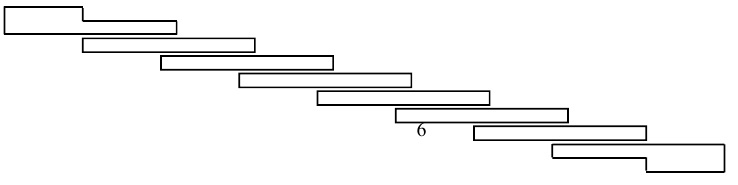
\includegraphics[width=0.46\textwidth]{figures/ref_filter_structure.png}
  \caption{滤波器二端口网络参量测量连接示意}
  \label{fig:ref-filter-test}
\end{figure}

平行耦合微带滤波器对外界环境较敏感。手指或金属片靠近时，耦合线附近的边缘场分布被改变，等效介电常数、谐振频率和耦合强度都会变化。这个特点正是外界干扰测试的物理基础：如果滤波器没有屏蔽结构，靠近导体或人体组织会显著改变 S21 曲线。

\section{实验过程}

\subsection{单端口反射校准}

微带线负载测量前，先连接射频电缆并进行单端口机械校准。校准过程依次接入开路器、短路器和匹配负载，使仪器把测量参考面移动到电缆末端。校准完成后，接入接近 50 $\Omega$ 的负载时，Smith 圆图上的轨迹应靠近中心区域。

\begin{figure}[!htbp]
  \centering
  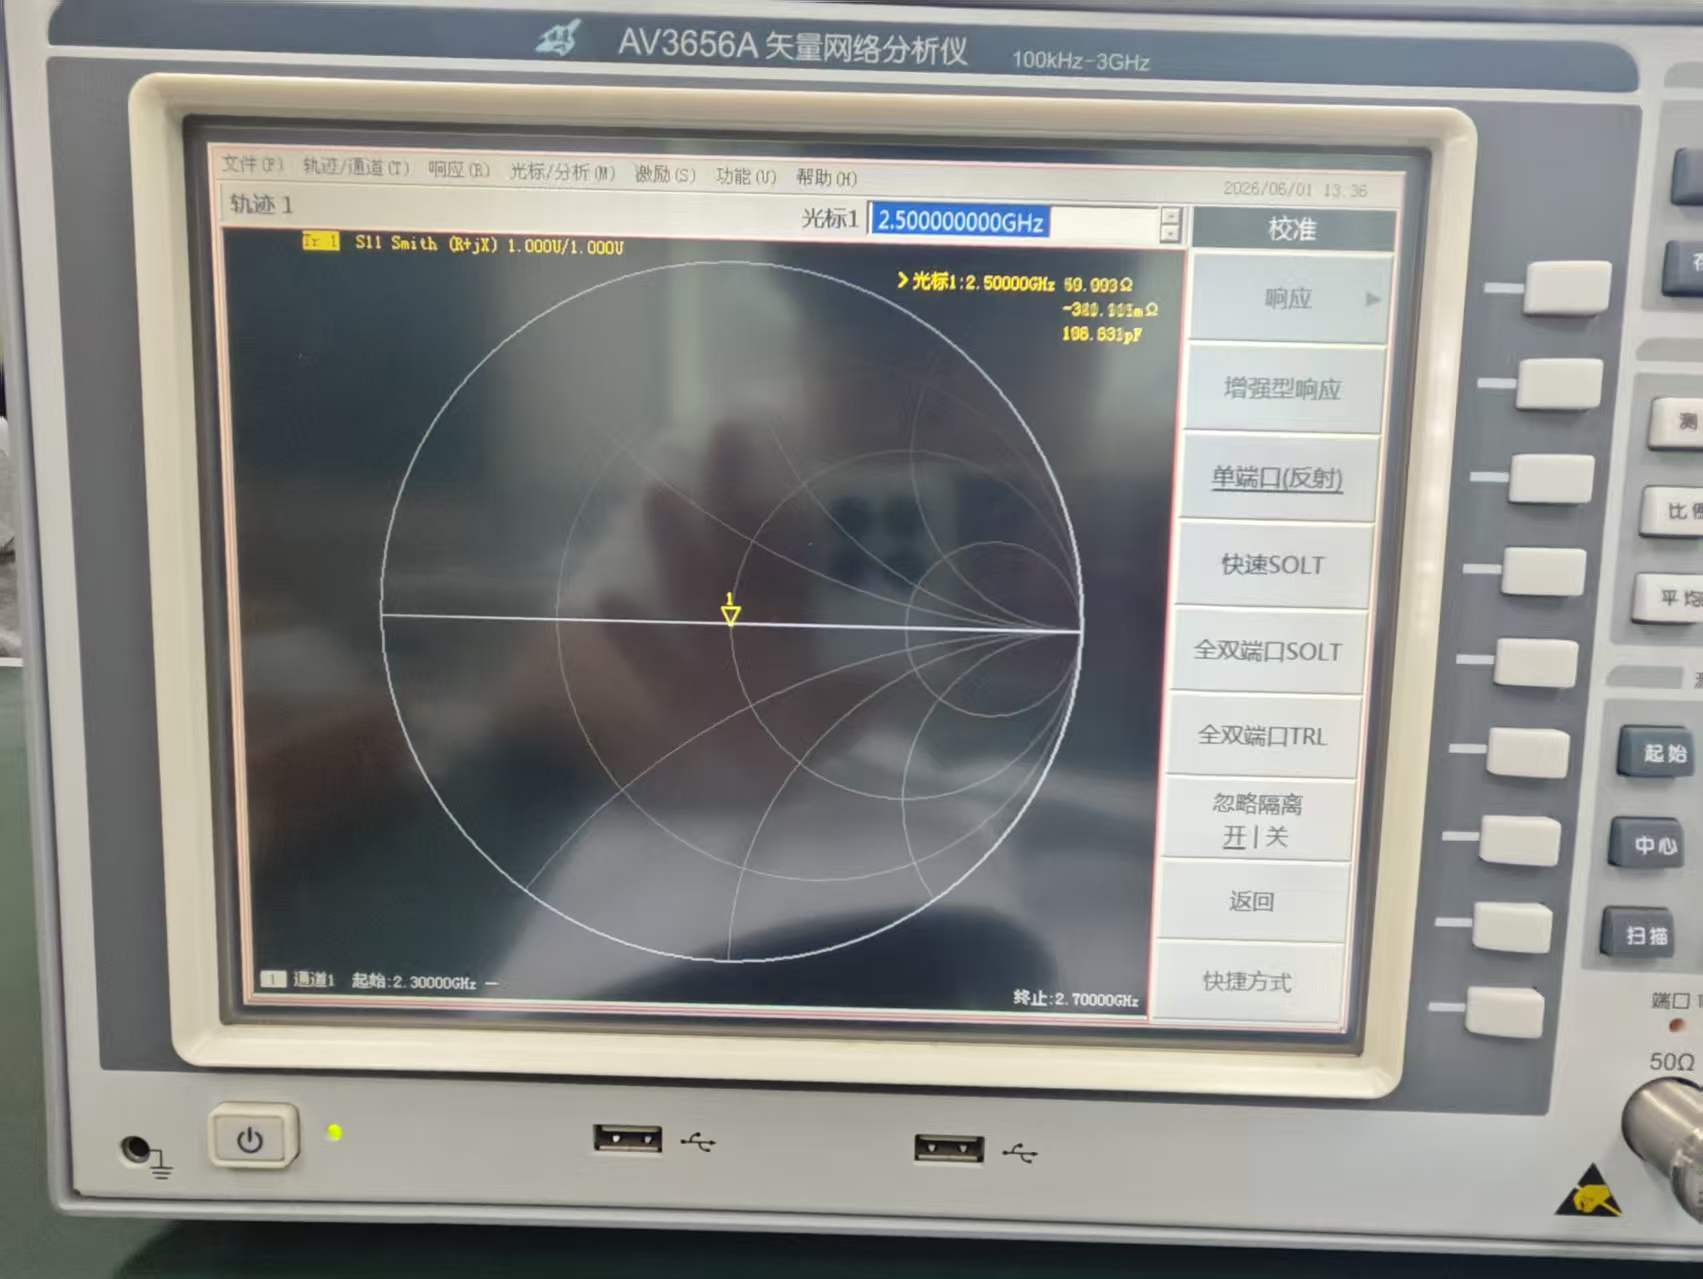
\includegraphics[width=0.64\textwidth]{figures/one_port_cal_done.png}
  \caption{单端口反射校准完成后的 Smith 圆图界面}
  \label{fig:one-port-cal}
\end{figure}

\subsection{微带传输线负载测量}

反射测量选择 S11 与 Smith 圆图格式，扫频范围设为 2.3 GHz 至 2.7 GHz。使用防静电镊子把贴片元件压接在微带线末端与接地铜箔之间，依次测量开路、短路、49.9 $\Omega$ 电阻、1 pF 电容和 3.3 nH 电感负载。对每种负载，在 2.3、2.4、2.5、2.6、2.7 GHz 放置光标并读取端口等效阻抗。

\subsection{天线测量}

天线直接通过 SMA-N 转接头连接到矢网端口，因此移除原射频电缆后重新进行单端口反射校准。扫频范围设为 1 GHz 至 3 GHz，记录 S11 对数幅度和驻波比曲线。测量中 S11 显示格式为对数幅度，数据处理中将其换算为线性反射系数进行分析。

\subsection{滤波器二端口测量}

滤波器传输特性测量选择 S21。校准时两个端口分别连接射频电缆和 N-SMA 转接头，再用直通接头连接，执行前向直通响应校准。随后移除直通接头并接入微带滤波器，读取 S21 对数幅度、相位和带宽搜索结果。

\section{实验数据与分析}

\subsection{微带传输线负载反射特性测量}

微带传输线负载测量采用 S11 Smith 圆图显示，系统参考阻抗为 $50\,\Omega$，频率范围为 2.3 GHz 至 2.7 GHz。理论比较中的反射系数按理想负载端计算，实测阻抗为矢网参考面向微带模块看进去的等效输入阻抗，因此两者不会完全相同。表中复反射系数按 $\Gamma=(Z_\mathrm{in}-50)/(Z_\mathrm{in}+50)$ 换算，差异主要来自微带线电长度、转接结构、贴片元件寄生参数和接触状态。

\subsubsection{开路负载}

\begin{figure}[H]
  \centering
  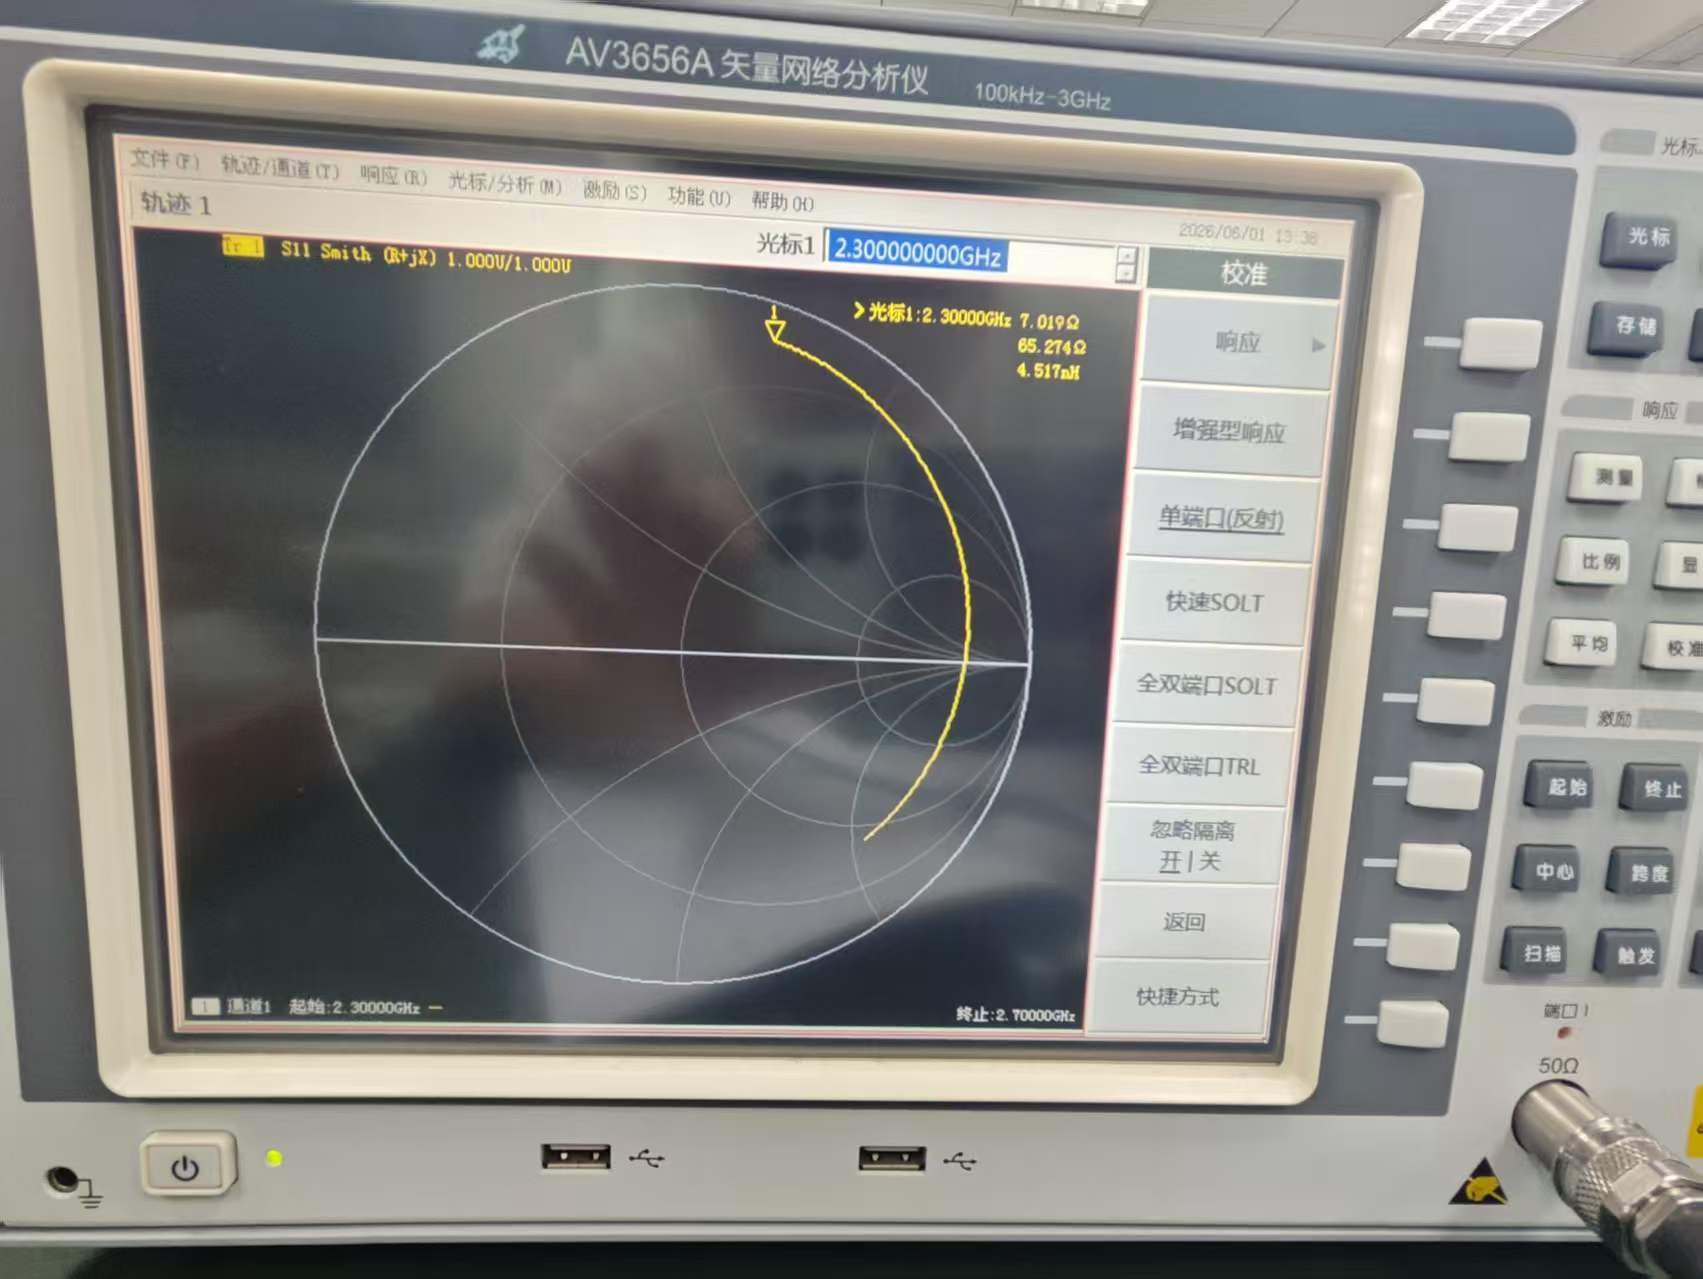
\includegraphics[width=0.48\textwidth]{figures/load_open.png}
  \caption{开路负载测量界面}
  \label{fig:load-open}
\end{figure}

\begin{table}[H]
  \centering
  \caption{开路负载反射特性数据}
  \label{tab:open-load}
  \small
  \begin{tabular}{ccccc}
    \toprule
    频率/GHz & 理想 $|\Gamma_L|$ & $Z_\mathrm{in}/\Omega$ & 实测 $\Gamma$ & $|\Gamma|$/VSWR \\
    \midrule
    2.3 & 1.000 & $7.02+j65.27$ & $0.241+j0.869$ & 0.902/19.35 \\
    2.4 & 1.000 & $16.80+j117.60$ & $0.635+j0.643$ & 0.904/19.73 \\
    2.5 & 1.000 & $286.40+j18.50$ & $0.704+j0.016$ & 0.704/5.75 \\
    2.6 & 1.000 & $18.20-j112.30$ & $0.605-j0.651$ & 0.888/16.91 \\
    2.7 & 1.000 & $7.50-j63.80$ & $0.221-j0.865$ & 0.893/17.61 \\
    \bottomrule
  \end{tabular}
\end{table}

理想开路端的反射系数模值为 1，驻波比趋于无穷大。实测 $|\Gamma|$ 大多接近 0.9，说明端接仍属于强反射状态；2.5 GHz 附近 $Z_\mathrm{in}$ 实部较大、虚部较小，接近半波长传输线把开路端变换为端口开路等效的情况。低频侧呈感性，高频侧转为容性，Smith 圆图轨迹体现了传输线电长度随频率变化导致的阻抗旋转。

\subsubsection{短路负载}

\begin{figure}[H]
  \centering
  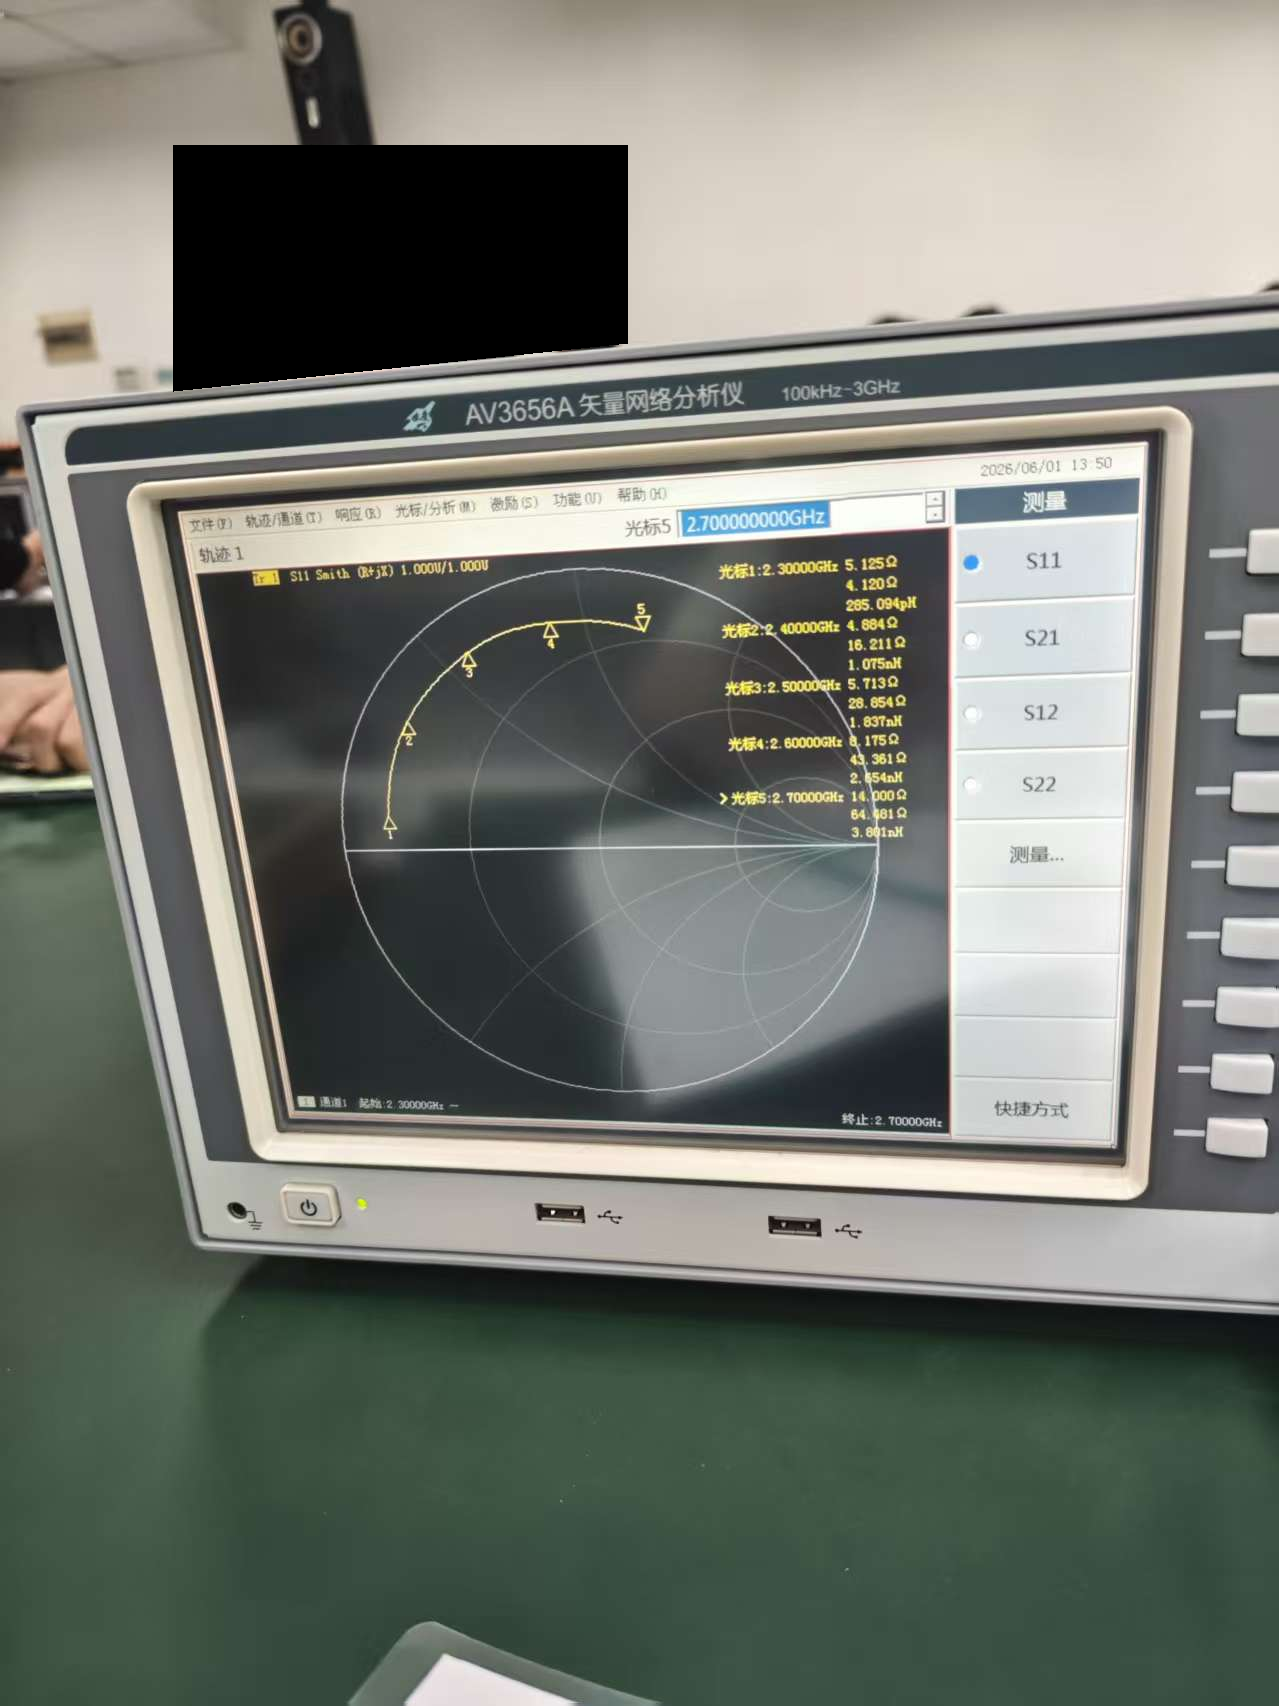
\includegraphics[width=0.48\textwidth]{figures/load_short.png}
  \caption{短路负载测量界面}
  \label{fig:load-short}
\end{figure}

\begin{table}[H]
  \centering
  \caption{短路负载反射特性数据}
  \label{tab:short-load}
  \small
  \begin{tabular}{ccccc}
    \toprule
    频率/GHz & 理想 $|\Gamma_L|$ & $Z_\mathrm{in}/\Omega$ & 实测 $\Gamma$ & $|\Gamma|$/VSWR \\
    \midrule
    2.3 & 1.000 & $5.13+j4.12$ & $-0.804+j0.135$ & 0.815/9.82 \\
    2.4 & 1.000 & $4.68+j16.21$ & $-0.681+j0.498$ & 0.844/11.81 \\
    2.5 & 1.000 & $5.71+j28.85$ & $-0.415+j0.733$ & 0.842/11.70 \\
    2.6 & 1.000 & $8.18+j41.36$ & $-0.142+j0.812$ & 0.824/10.37 \\
    2.7 & 1.000 & $11.00+j64.48$ & $0.226+j0.818$ & 0.849/12.24 \\
    \bottomrule
  \end{tabular}
\end{table}

理想短路端满足 $Z_L=0$，反射系数为 $-1$，反射强度同样接近全反射。实测阻抗实部较小，虚部随频率升高逐渐增大，表现为经过微带线和连接结构后的感性输入阻抗。$|\Gamma|$ 保持在 0.815 至 0.849 之间，驻波比较大，符合短路负载强反射的特征。

\subsubsection{49.9 $\Omega$ 电阻负载}

\begin{figure}[H]
  \centering
  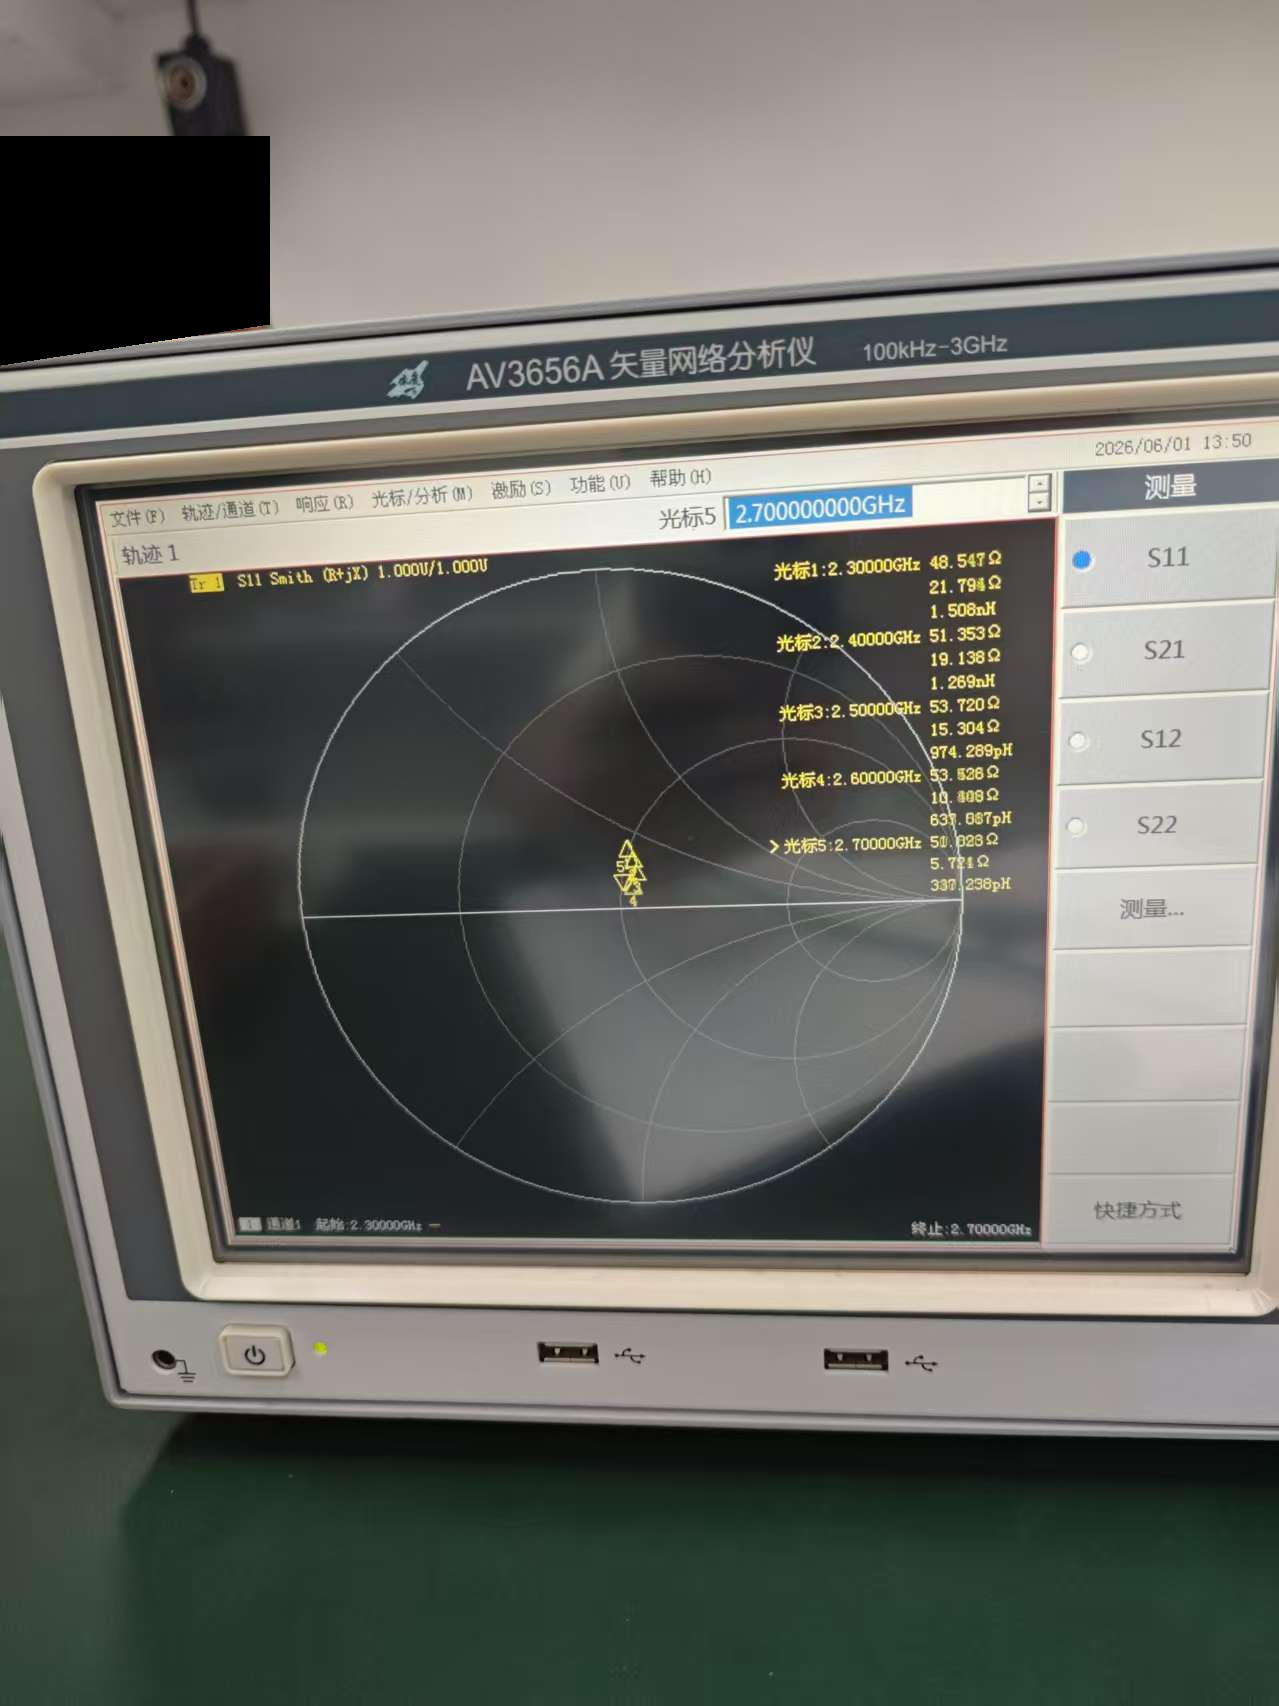
\includegraphics[width=0.48\textwidth]{figures/load_match.png}
  \caption{49.9 $\Omega$ 电阻负载测量界面}
  \label{fig:load-match}
\end{figure}

\begin{table}[H]
  \centering
  \caption{49.9 $\Omega$ 电阻负载反射特性数据}
  \label{tab:match-load}
  \small
  \begin{tabular}{ccccc}
    \toprule
    频率/GHz & 理论 $|\Gamma_L|$ & $Z_\mathrm{in}/\Omega$ & 实测 $\Gamma$ & $|\Gamma|$/VSWR \\
    \midrule
    2.3 & 0.001 & $48.55+j21.79$ & $0.033+j0.214$ & 0.216/1.55 \\
    2.4 & 0.001 & $51.35+j19.14$ & $0.047+j0.180$ & 0.186/1.46 \\
    2.5 & 0.001 & $53.72+j15.30$ & $0.056+j0.139$ & 0.150/1.35 \\
    2.6 & 0.001 & $53.63+j10.40$ & $0.045+j0.096$ & 0.106/1.24 \\
    2.7 & 0.001 & $50.83+j5.72$ & $0.011+j0.056$ & 0.057/1.12 \\
    \bottomrule
  \end{tabular}
\end{table}

实际接入电阻为 49.9 $\Omega$，相对于 $50\,\Omega$ 系统的理想负载反射系数约为 0.001，理论上应非常接近匹配。实测结果中阻抗实部接近 $50\,\Omega$，虚部随频率升高逐渐减小，Smith 圆图轨迹向中心靠近。2.7 GHz 处 $|\Gamma|$ 仅约 0.057，VSWR 约 1.12，为各类负载中匹配效果最好的状态；低频端仍有一定虚部，说明微带过渡和负载压接结构引入了附加电抗。

\subsubsection{1 pF 电容负载}

\begin{figure}[H]
  \centering
  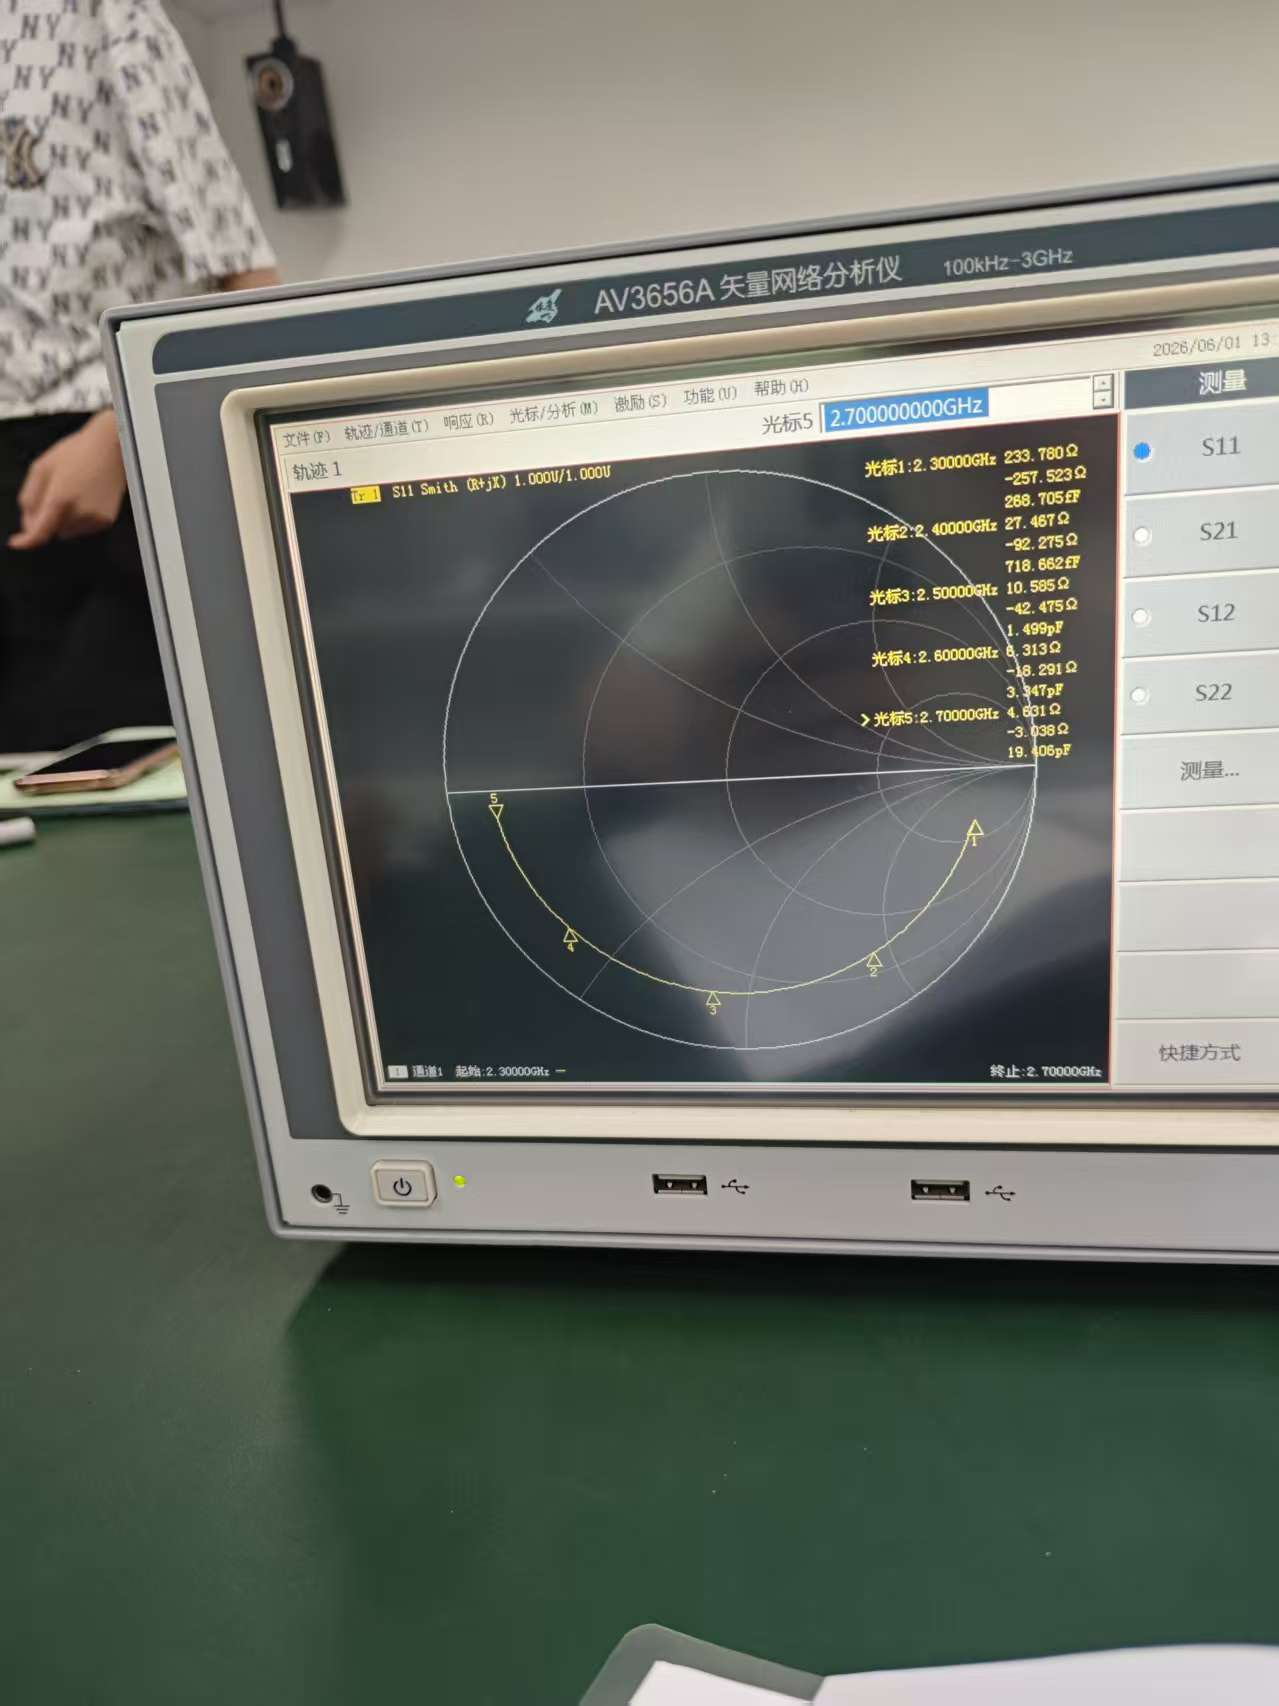
\includegraphics[width=0.48\textwidth]{figures/load_cap.png}
  \caption{1 pF 电容负载测量界面}
  \label{fig:load-cap}
\end{figure}

\begin{table}[H]
  \centering
  \caption{1 pF 电容负载反射特性数据}
  \label{tab:cap-load}
  \scriptsize
  \setlength{\tabcolsep}{3pt}
  \begin{tabular}{cccccc}
    \toprule
    频率/GHz & 理想 $X_C/\Omega$ & $Z_\mathrm{in}/\Omega$ & 实测 $\Gamma$ & $|\Gamma|$/VSWR & $C_\mathrm{eq}$ \\
    \midrule
    2.3 & -69.20 & $233.78-j257.52$ & $0.807-j0.175$ & 0.826/10.47 & 0.269 pF \\
    2.4 & -66.31 & $27.47-j92.27$ & $0.466-j0.636$ & 0.788/8.45 & 0.719 pF \\
    2.5 & -63.66 & $10.59-j42.48$ & $-0.107-j0.776$ & 0.783/8.22 & 1.499 pF \\
    2.6 & -61.21 & $8.31-j18.29$ & $-0.561-j0.490$ & 0.745/6.84 & 3.347 pF \\
    2.7 & -58.95 & $4.60-j3.04$ & $-0.826-j0.102$ & 0.832/10.91 & 19.406 pF \\
    \bottomrule
  \end{tabular}
\end{table}

理想 1 pF 电容在本频段内呈几十欧姆量级的容性电抗，端接在 $50\,\Omega$ 系统上时不会形成匹配。实测输入阻抗整体位于 Smith 圆图容性区域，$|\Gamma|$ 多数大于 0.78，说明反射较强。2.5 GHz 附近端口等效电容为 1.499 pF，与标称值量级接近；继续升高频率后，接触结构、焊盘和微带端部场的寄生效应更明显，端口等效电容快速增大，不能再把测得结果简单看成贴片电容本体。

\subsubsection{3.3 nH 电感负载}

\begin{figure}[H]
  \centering
  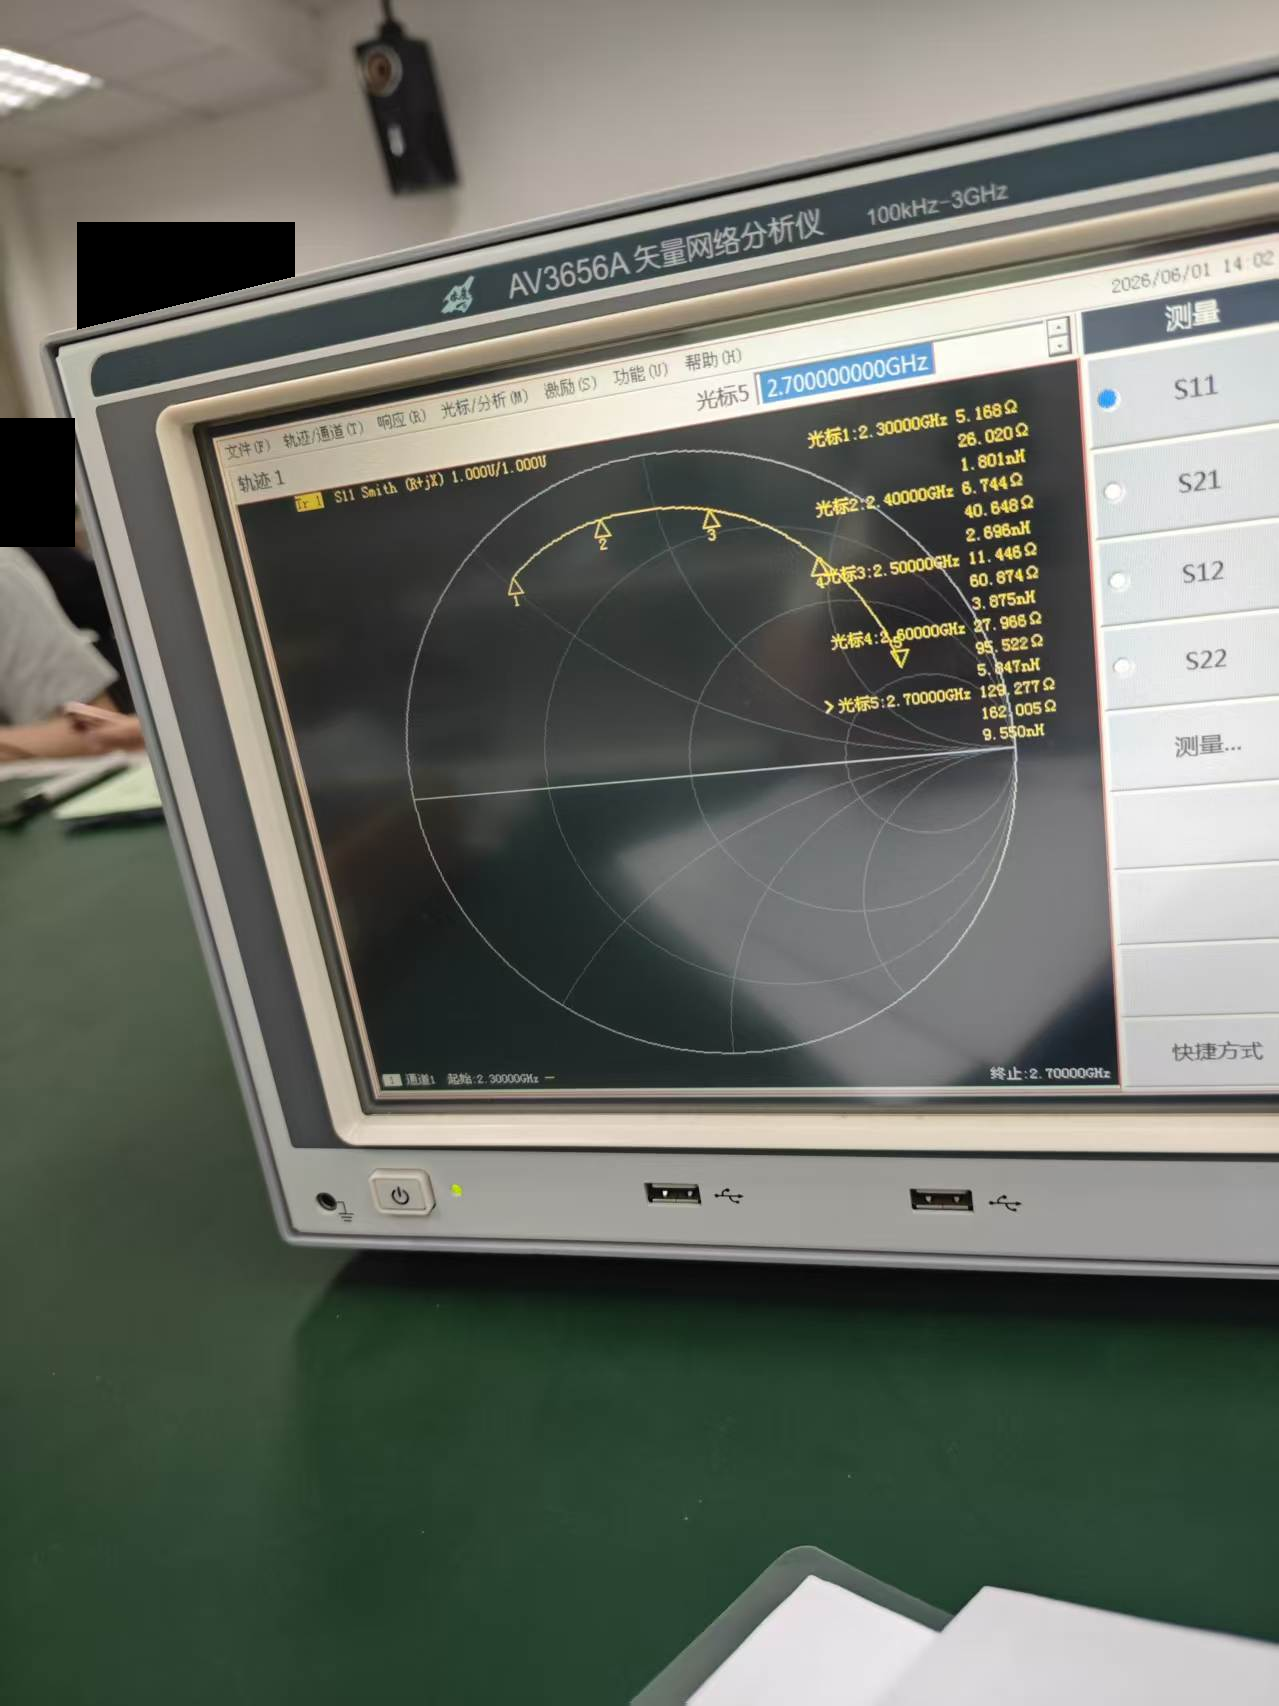
\includegraphics[width=0.48\textwidth]{figures/load_ind.png}
  \caption{3.3 nH 电感负载测量界面}
  \label{fig:load-ind}
\end{figure}

\begin{table}[H]
  \centering
  \caption{3.3 nH 电感负载反射特性数据}
  \label{tab:ind-load}
  \scriptsize
  \setlength{\tabcolsep}{3pt}
  \begin{tabular}{cccccc}
    \toprule
    频率/GHz & 理想 $X_L/\Omega$ & $Z_\mathrm{in}/\Omega$ & 实测 $\Gamma$ & $|\Gamma|$/VSWR & $L_\mathrm{eq}$ \\
    \midrule
    2.3 & 47.69 & $5.17+j26.02$ & $-0.483+j0.699$ & 0.850/12.32 & 1.801 nH \\
    2.4 & 49.76 & $6.74+j40.65$ & $-0.165+j0.834$ & 0.850/12.37 & 2.696 nH \\
    2.5 & 51.84 & $11.45+j60.67$ & $0.176+j0.814$ & 0.832/10.94 & 3.875 nH \\
    2.6 & 53.91 & $27.97+j95.52$ & $0.487+j0.628$ & 0.795/8.76 & 5.847 nH \\
    2.7 & 55.98 & $129.28+j162.01$ & $0.693+j0.277$ & 0.746/6.89 & 9.550 nH \\
    \bottomrule
  \end{tabular}
\end{table}

理想 3.3 nH 电感的电抗从 47.69 $\Omega$ 增至 55.98 $\Omega$，属于感性非匹配端接。实测点均位于感性区域，2.4 GHz 至 2.5 GHz 附近端口等效电感与标称量级较接近；2.7 GHz 处等效电感明显增大，同时 $Z_\mathrm{in}$ 实部也升高，反映出高频寄生损耗、贴片元件自谐振趋势和压接结构综合作用。与电容负载类似，这里的等效电感应理解为端口参考面处的整体等效量。

\subsection{天线测量}

\begin{figure}[H]
  \centering
  \begin{subfigure}[b]{0.47\textwidth}
    \centering
    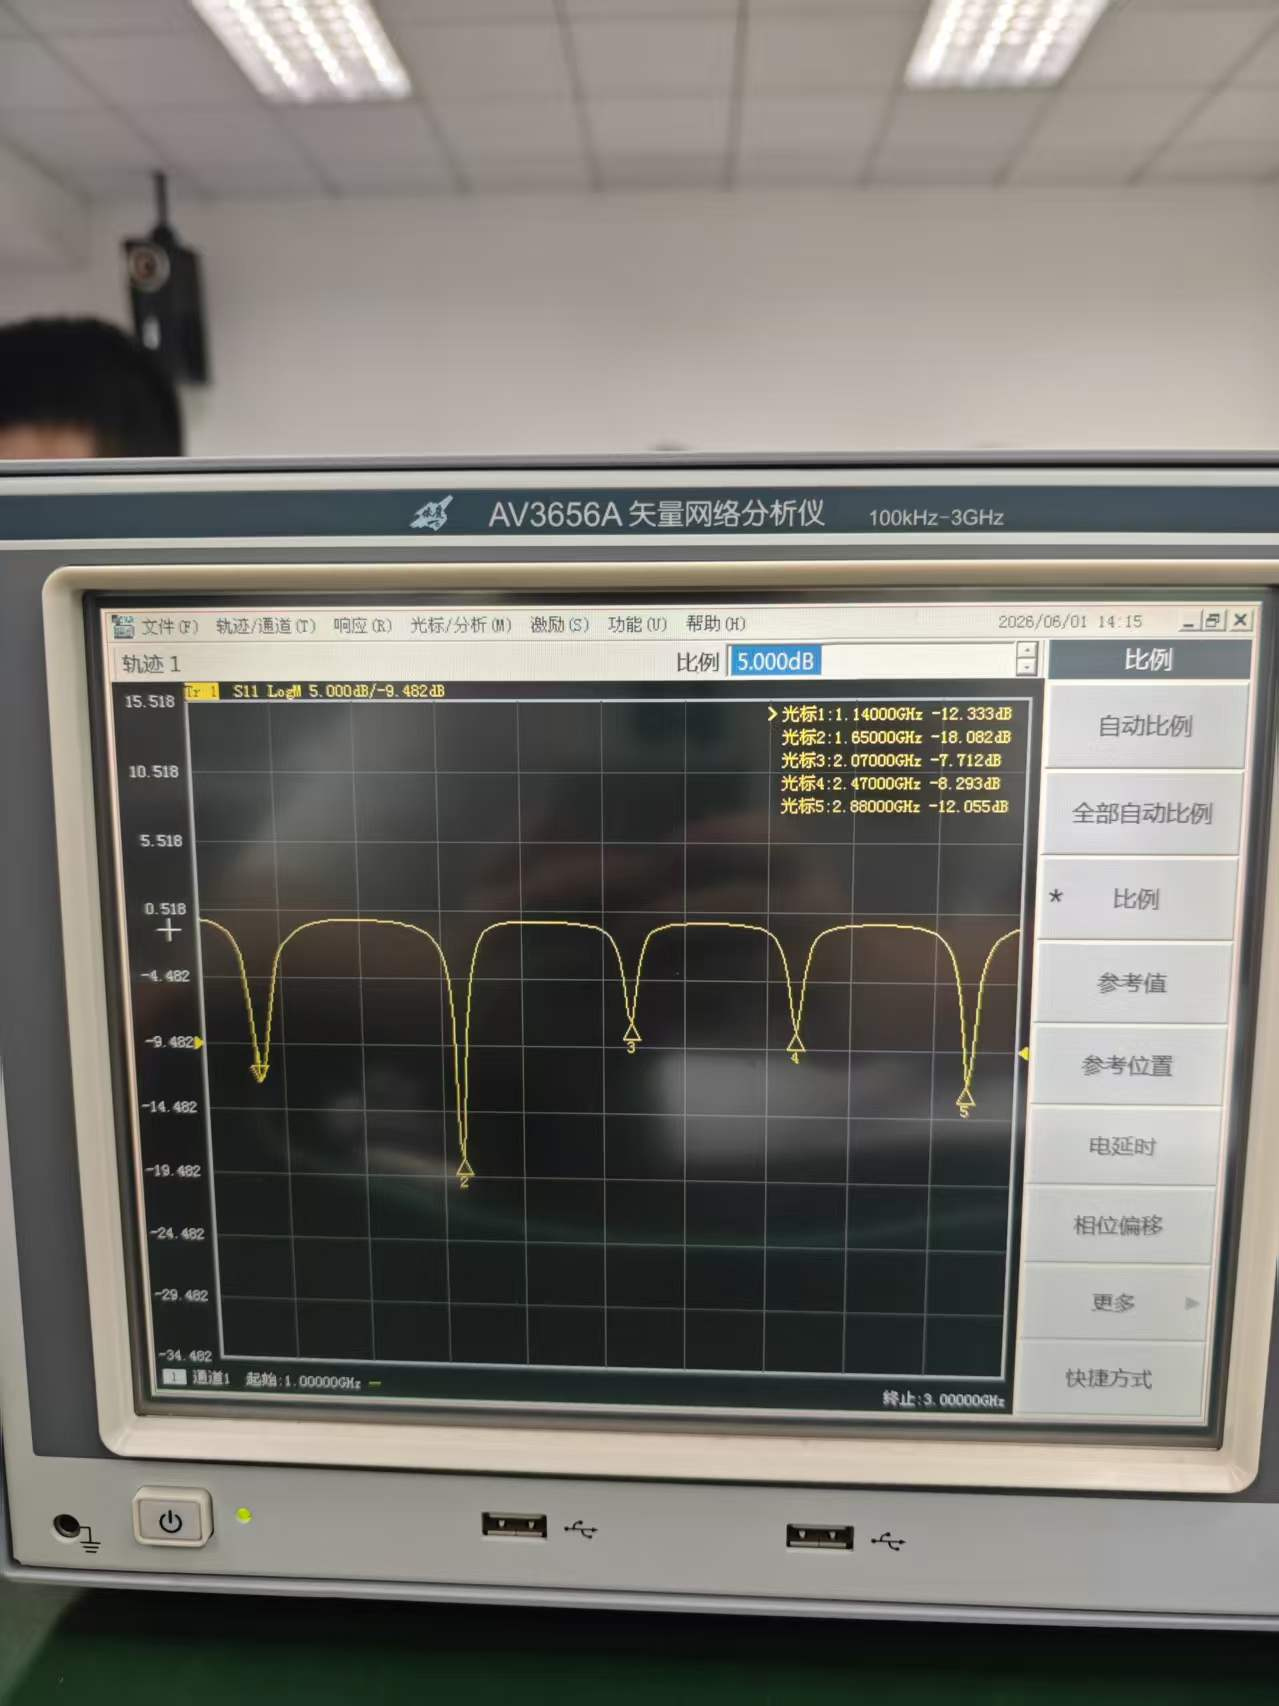
\includegraphics[width=\textwidth]{figures/antenna_s11_log.png}
    \caption{天线 S11 对数幅度}
  \end{subfigure}
  \hfill
  \begin{subfigure}[b]{0.47\textwidth}
    \centering
    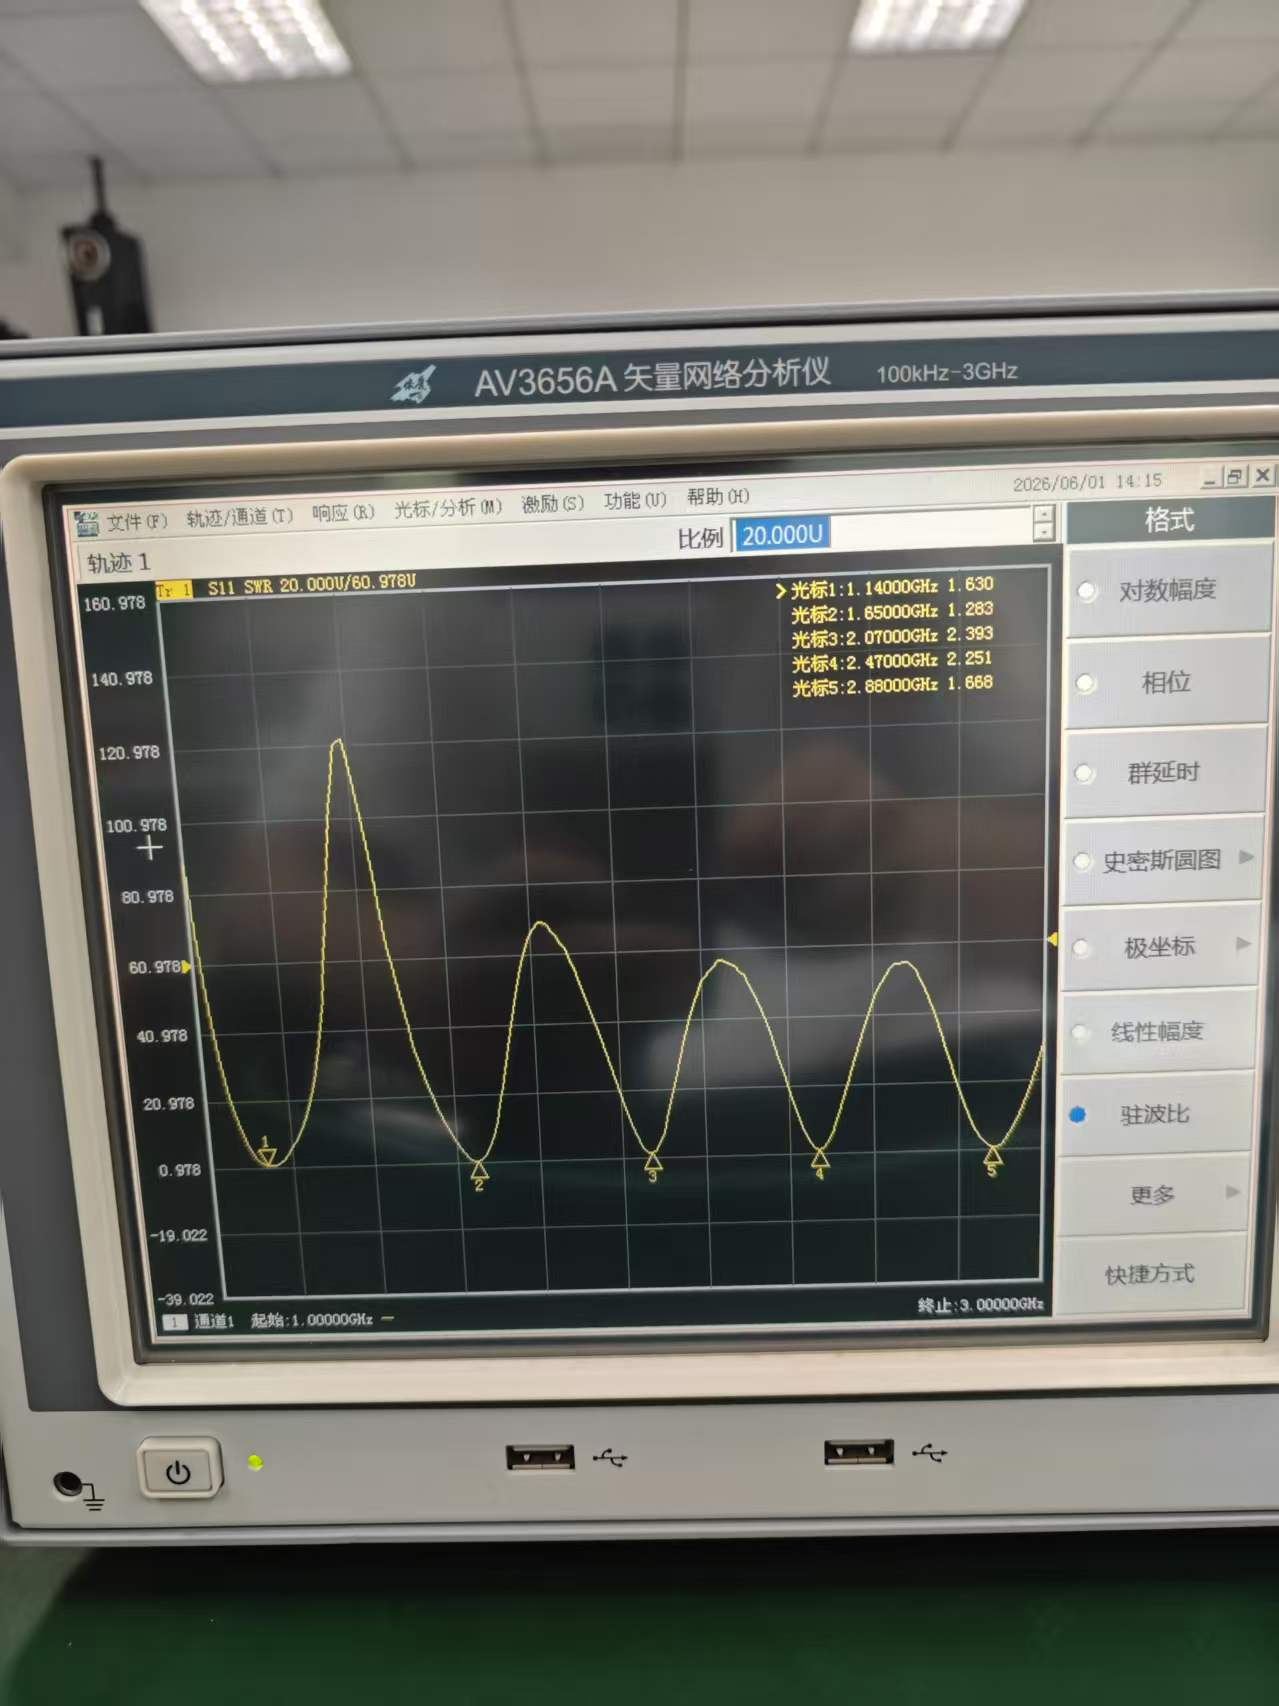
\includegraphics[width=\textwidth]{figures/antenna_vswr.png}
    \caption{天线驻波比}
  \end{subfigure}
  \caption{天线反射特性与驻波比测量结果}
  \label{fig:antenna-results}
\end{figure}

\begin{table}[H]
  \centering
  \caption{天线 S11 与驻波比测量结果}
  \label{tab:antenna}
  \small
  \begin{tabular}{ccccc}
    \toprule
    频率/GHz & $S_{11}$/dB & 换算 $|\Gamma|$ & VSWR 读数 & 匹配评价 \\
    \midrule
    1.14 & -12.333 & 0.242 & 1.630 & 较好 \\
    1.65 & -18.082 & 0.125 & 1.283 & 最佳 \\
    2.07 & -7.712 & 0.412 & 2.393 & 一般 \\
    2.47 & -8.293 & 0.385 & 2.251 & 一般 \\
    2.86 & -12.055 & 0.250 & 1.668 & 较好 \\
    \bottomrule
  \end{tabular}
\end{table}

天线 S11 采用对数幅度显示，线性反射系数按 $|\Gamma|=10^{S_{11,\mathrm{dB}}/20}$ 换算。由表 \ref{tab:antenna} 可见，1.65 GHz 处 $S_{11}=-18.082\,\mathrm{dB}$，VSWR 为 1.283，匹配最好；2.86 GHz 附近也有较好的匹配点。2.47 GHz 处 VSWR 约 2.251，说明该天线在 2.4 GHz 附近可工作但匹配不够理想，若用于该频段系统，仍需结合实际辐射效率和匹配网络进一步判断。

\subsection{微带耦合滤波器网络参量测量}

\subsubsection{S21 幅频与相频特性}

\begin{figure}[H]
  \centering
  \begin{subfigure}[b]{0.47\textwidth}
    \centering
    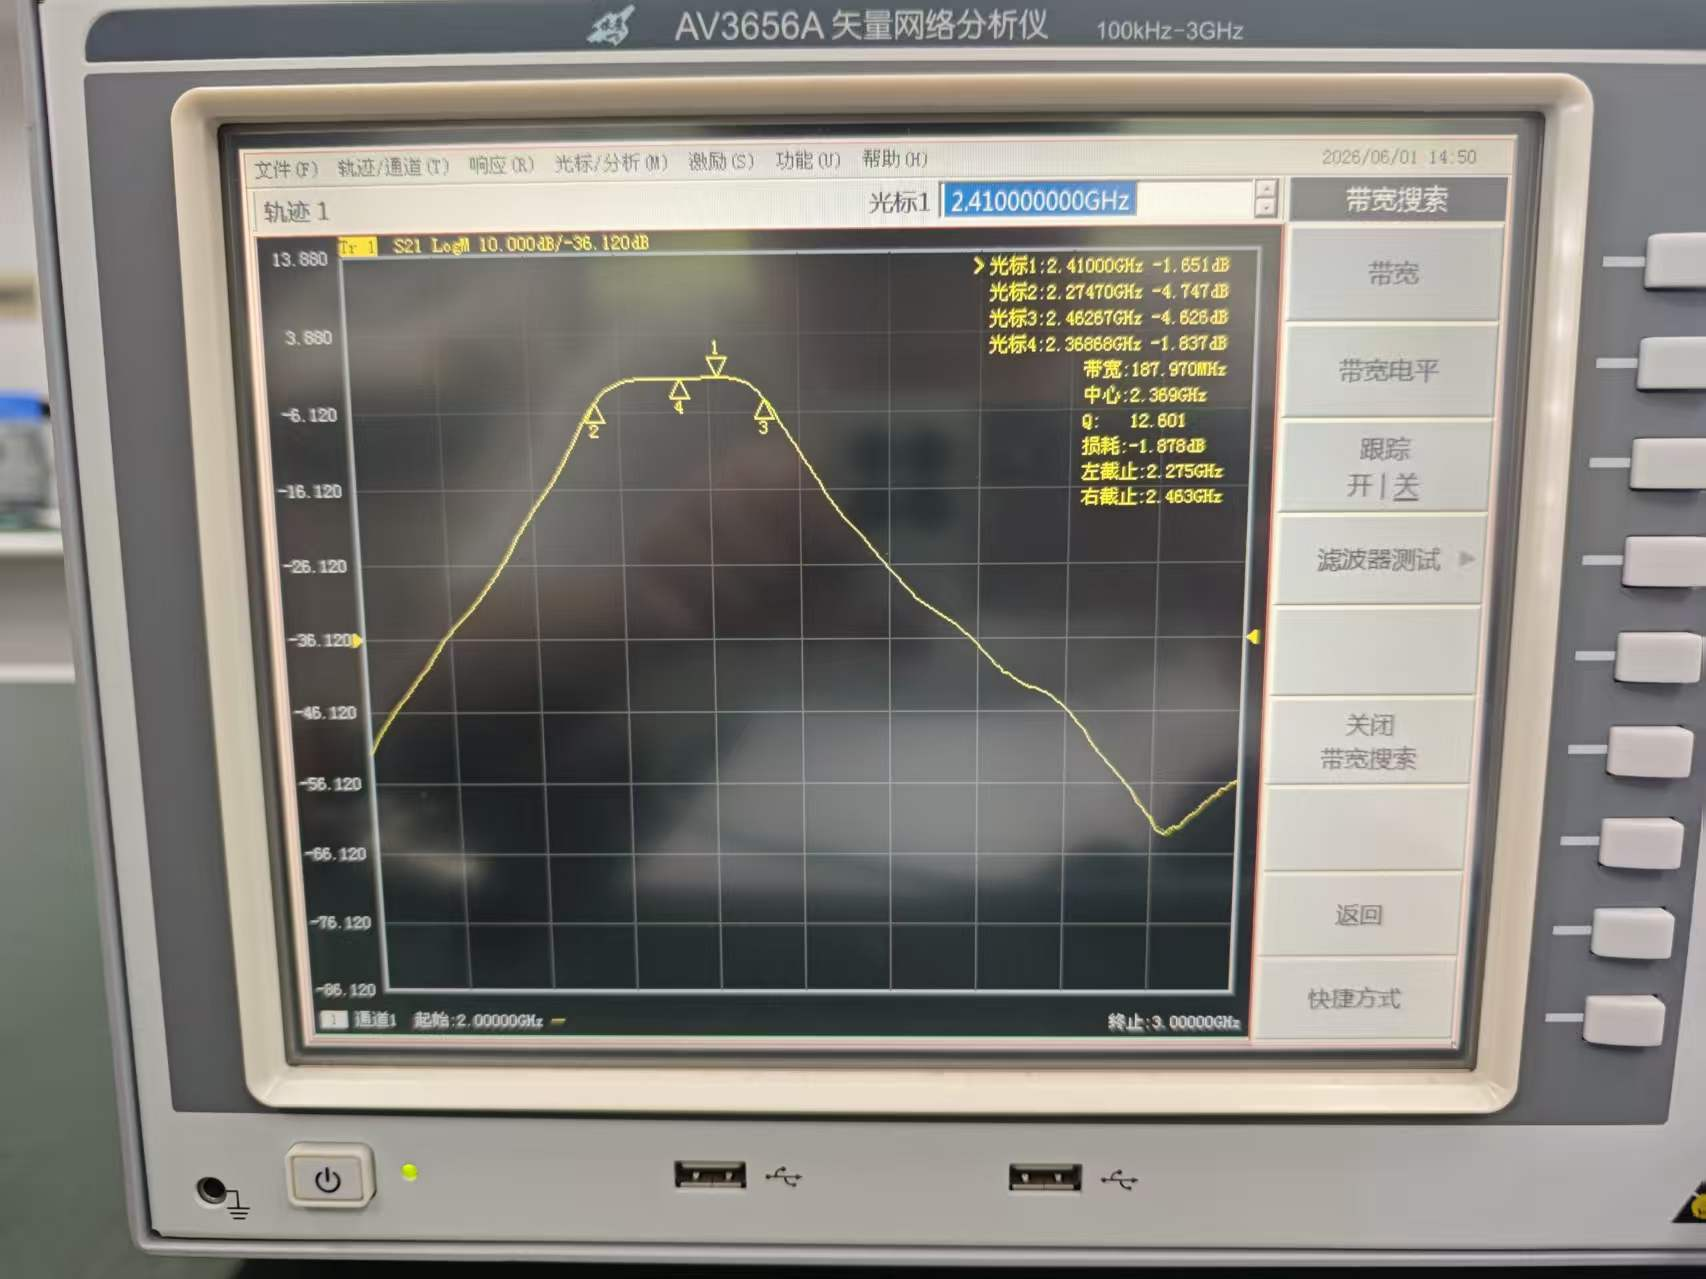
\includegraphics[width=\textwidth]{figures/filter_bandwidth.png}
    \caption{S21 幅度与带宽搜索}
  \end{subfigure}
  \hfill
  \begin{subfigure}[b]{0.47\textwidth}
    \centering
    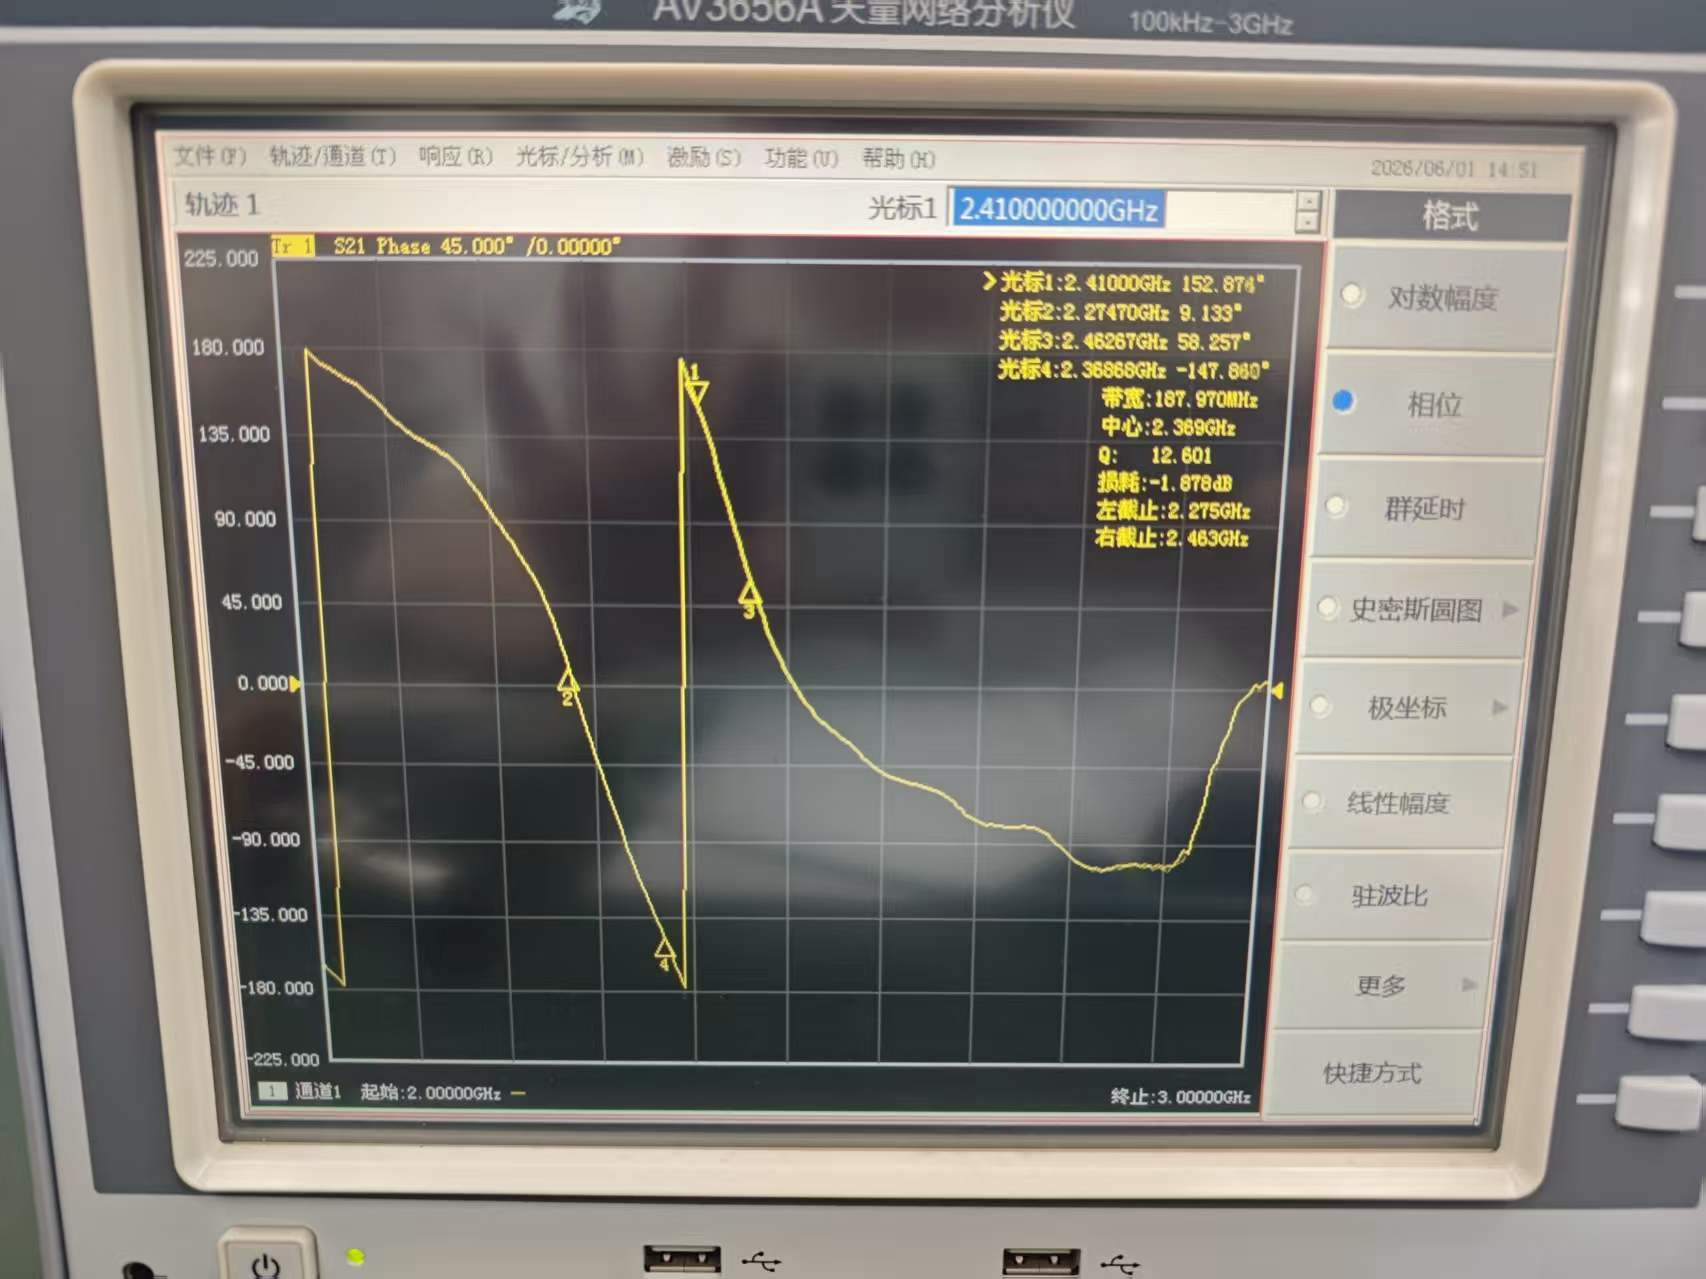
\includegraphics[width=\textwidth]{figures/filter_phase.png}
    \caption{S21 相位曲线}
  \end{subfigure}
  \caption{微带耦合滤波器 S21 测量结果}
  \label{fig:filter-results}
\end{figure}

\begin{table}[H]
  \centering
  \caption{滤波器 S21 带宽搜索数据}
  \label{tab:filter}
  \small
  \begin{tabular}{cccc}
    \toprule
    光标 & 频率/GHz & $S_{21}$/dB & 相位/度 \\
    \midrule
    1 & 2.41000 & -1.651 & 152.874 \\
    2 & 2.27470 & -4.747 & 9.133 \\
    3 & 2.46267 & -4.620 & 50.257 \\
    4 & 2.36868 & -1.837 & -147.880 \\
    \bottomrule
  \end{tabular}
\end{table}

带宽搜索结果给出中心频率 $f_0=2.369\,\mathrm{GHz}$，左、右 3 dB 频率分别约为 2.275 GHz 和 2.463 GHz，3 dB 带宽 $\Delta f=187.970\,\mathrm{MHz}$，品质因数 $Q=12.601$，中心附近插入损耗约 $1.878\,\mathrm{dB}$。2.36868 GHz 与 2.41000 GHz 处幅度差约 0.19 dB，通带顶部较平坦。相位曲线在通带内快速变化，显示中出现 $-180^\circ$ 与 $+180^\circ$ 之间的包裹跳变，这是相位显示范围造成的读数形式，不代表滤波器物理相位不连续。

\subsubsection{外界干扰影响测试}

\begin{figure}[H]
  \centering
  \begin{subfigure}[b]{0.47\textwidth}
    \centering
    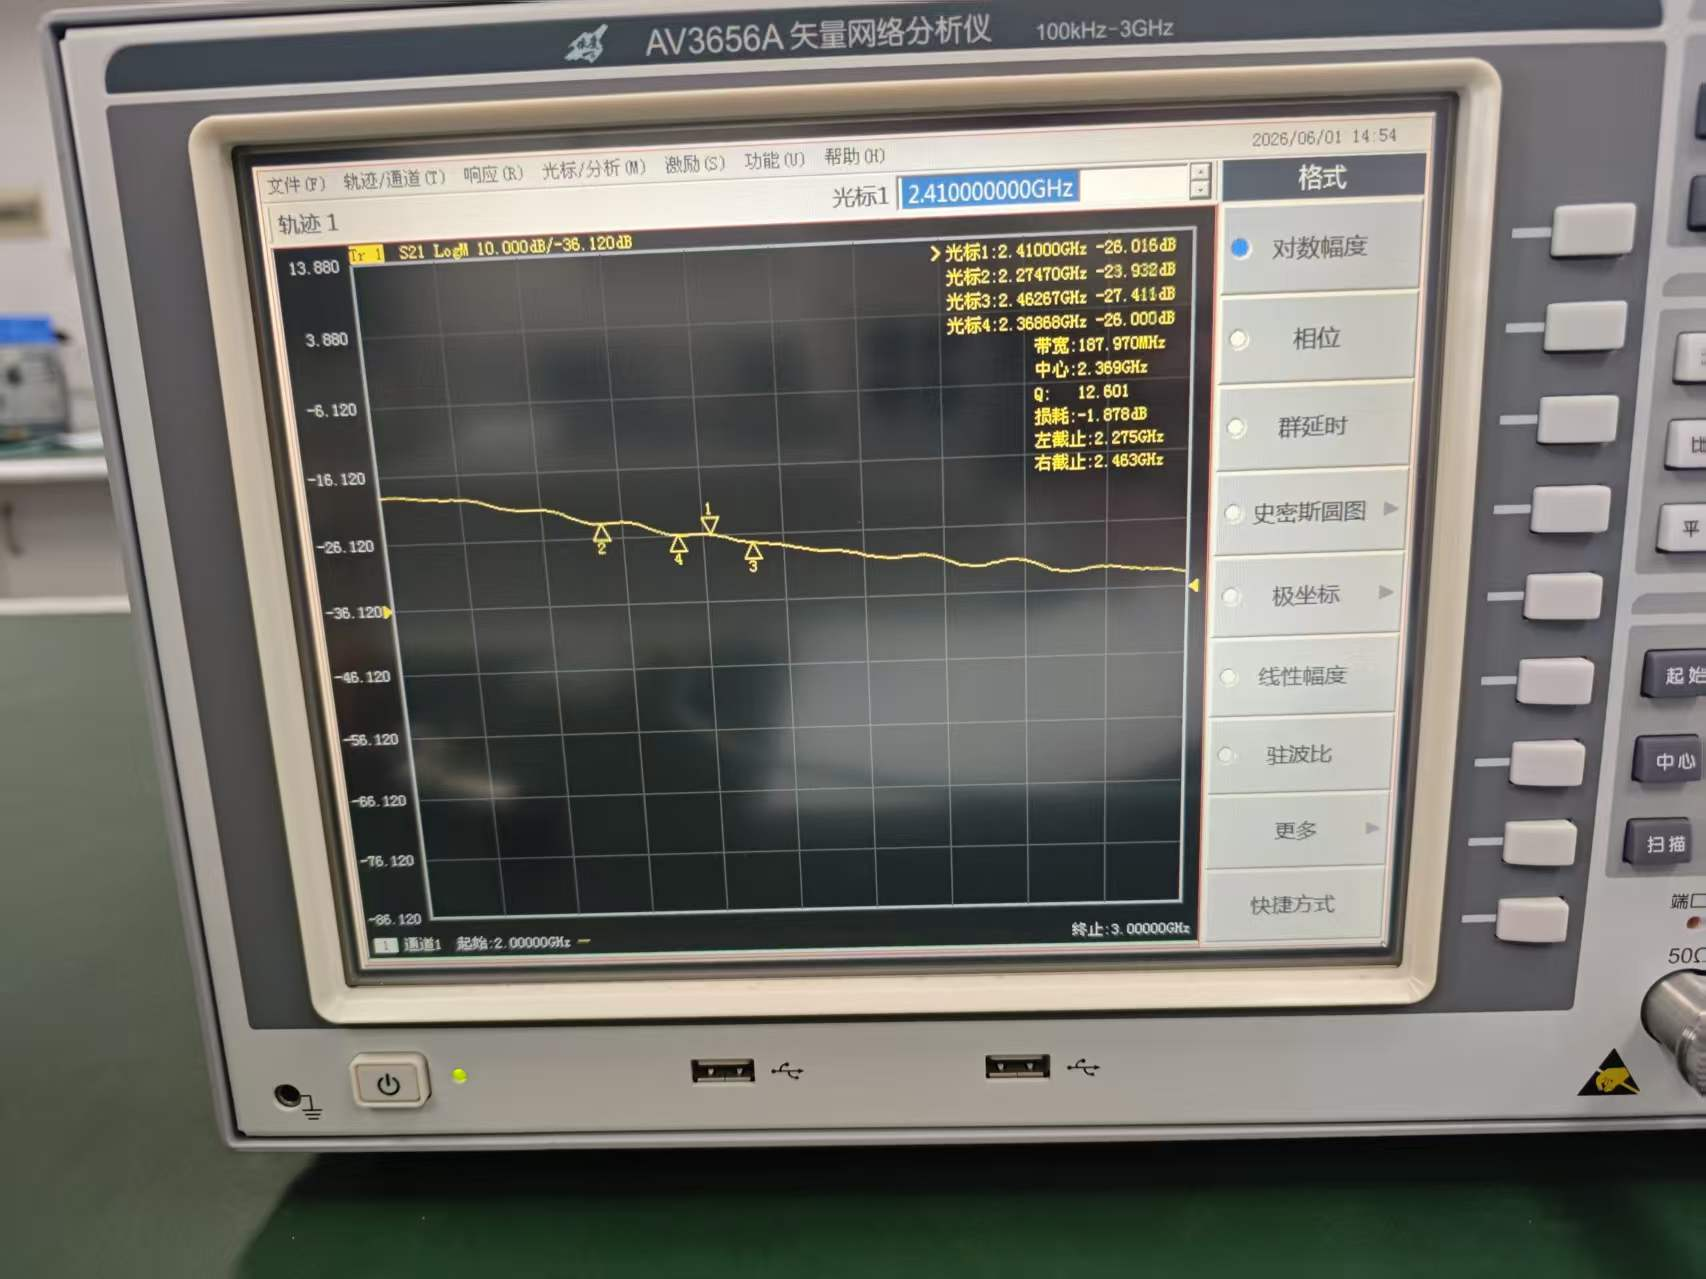
\includegraphics[width=\textwidth]{figures/interference_log1.png}
    \caption{扰动状态 1}
  \end{subfigure}
  \hfill
  \begin{subfigure}[b]{0.47\textwidth}
    \centering
    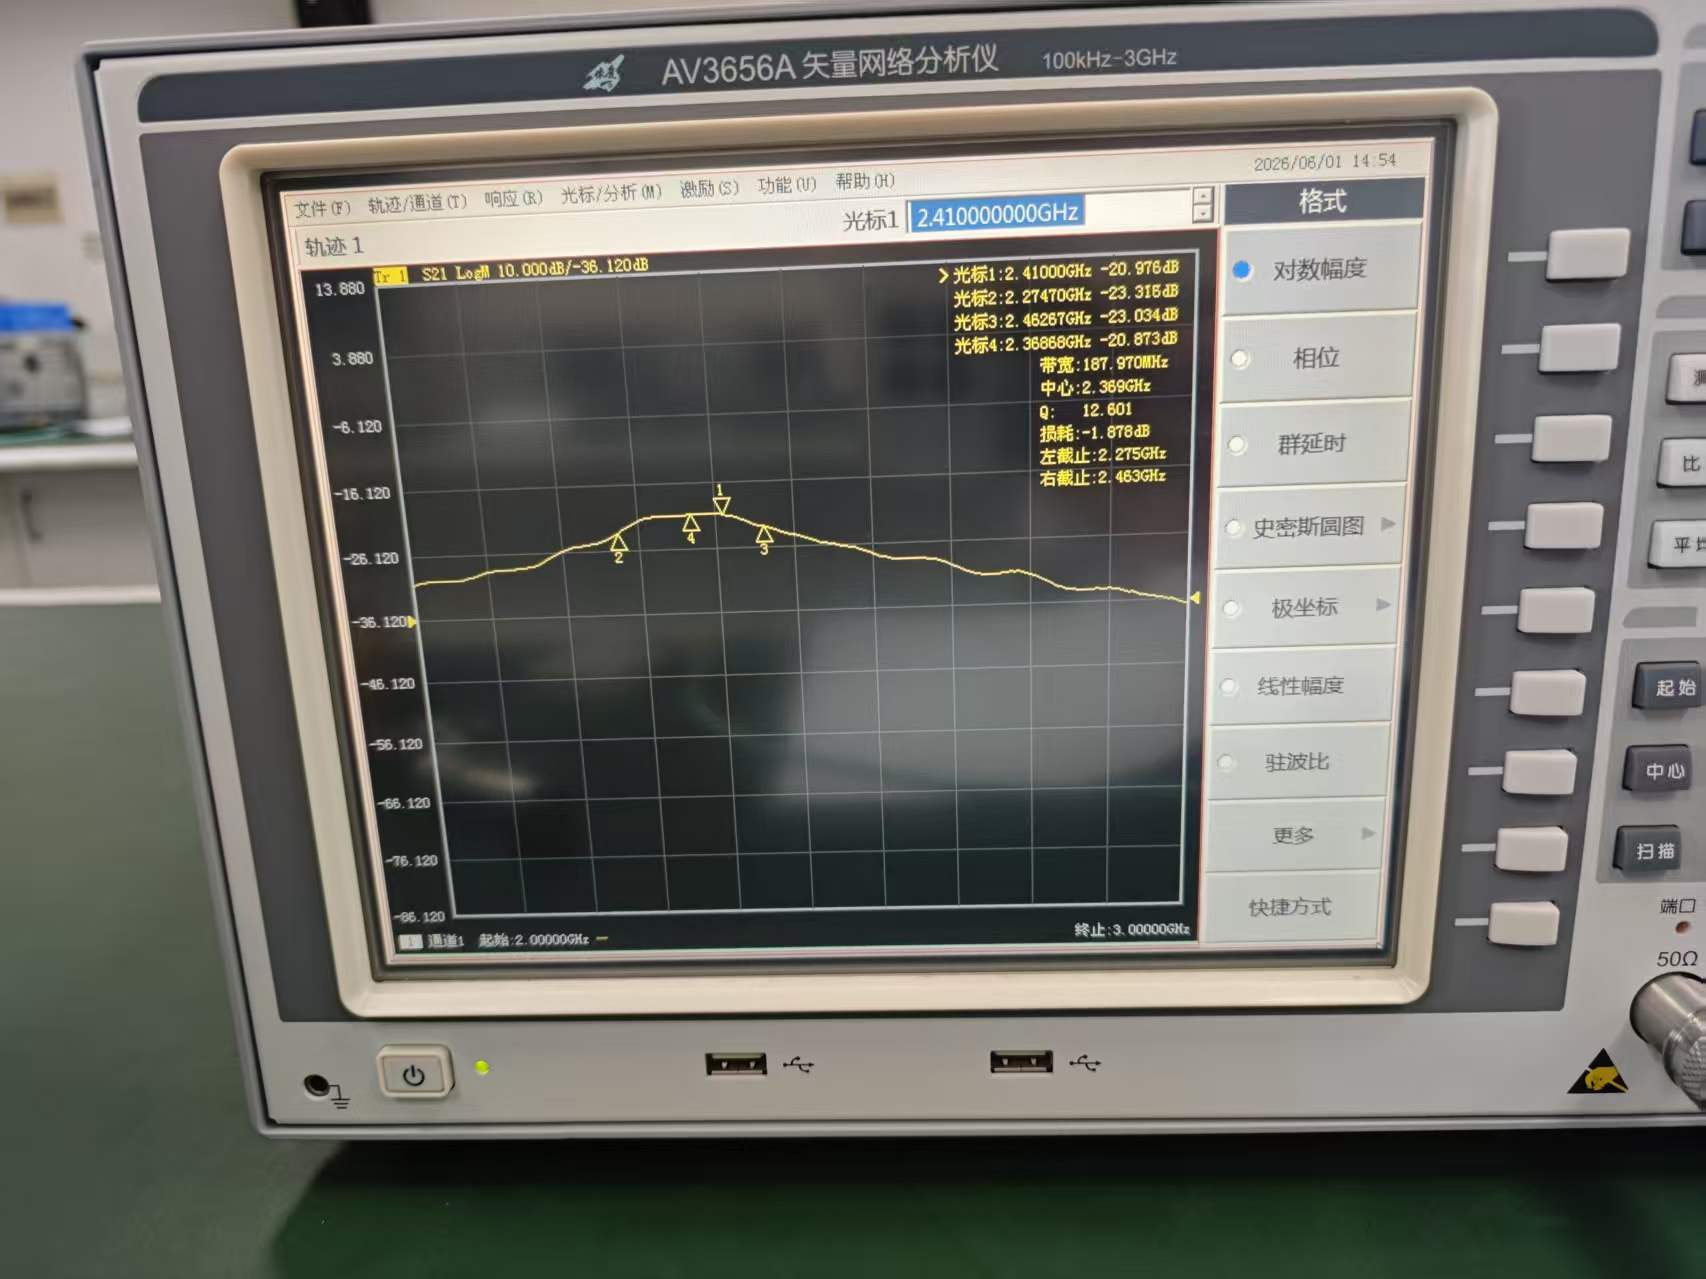
\includegraphics[width=\textwidth]{figures/interference_log2.png}
    \caption{扰动状态 2}
  \end{subfigure}
  \caption{外界扰动对滤波器 S21 对数幅度的影响}
  \label{fig:interference-log}
\end{figure}

\begin{table}[H]
  \centering
  \caption{外界扰动前后 S21 读数对比}
  \label{tab:interference}
  \small
  \begin{tabular}{cccc}
    \toprule
    频率/GHz & 正常 S21/dB & 扰动状态 1/dB & 扰动状态 2/dB \\
    \midrule
    2.27470 & -4.747 & -23.932 & -23.315 \\
    2.36868 & -1.837 & -26.000 & -20.873 \\
    2.41000 & -1.651 & -26.016 & -20.976 \\
    2.46267 & -4.620 & -27.411 & -23.034 \\
    \bottomrule
  \end{tabular}
\end{table}

外界物体靠近后，原通带频点处的 S21 明显下降。以 2.36868 GHz 为例，正常状态下为 $-1.837\,\mathrm{dB}$，扰动状态 1 降至 $-26.000\,\mathrm{dB}$，扰动状态 2 降至 $-20.873\,\mathrm{dB}$，额外衰减约 19 dB 至 24 dB。平行耦合微带滤波器的边缘场分布在空气中，附近介质或导体会改变等效介电常数和耦合强度，因此通带幅度、中心频率和带宽都会受到影响。

\begin{figure}[H]
  \centering
  \begin{subfigure}[b]{0.45\textwidth}
    \centering
    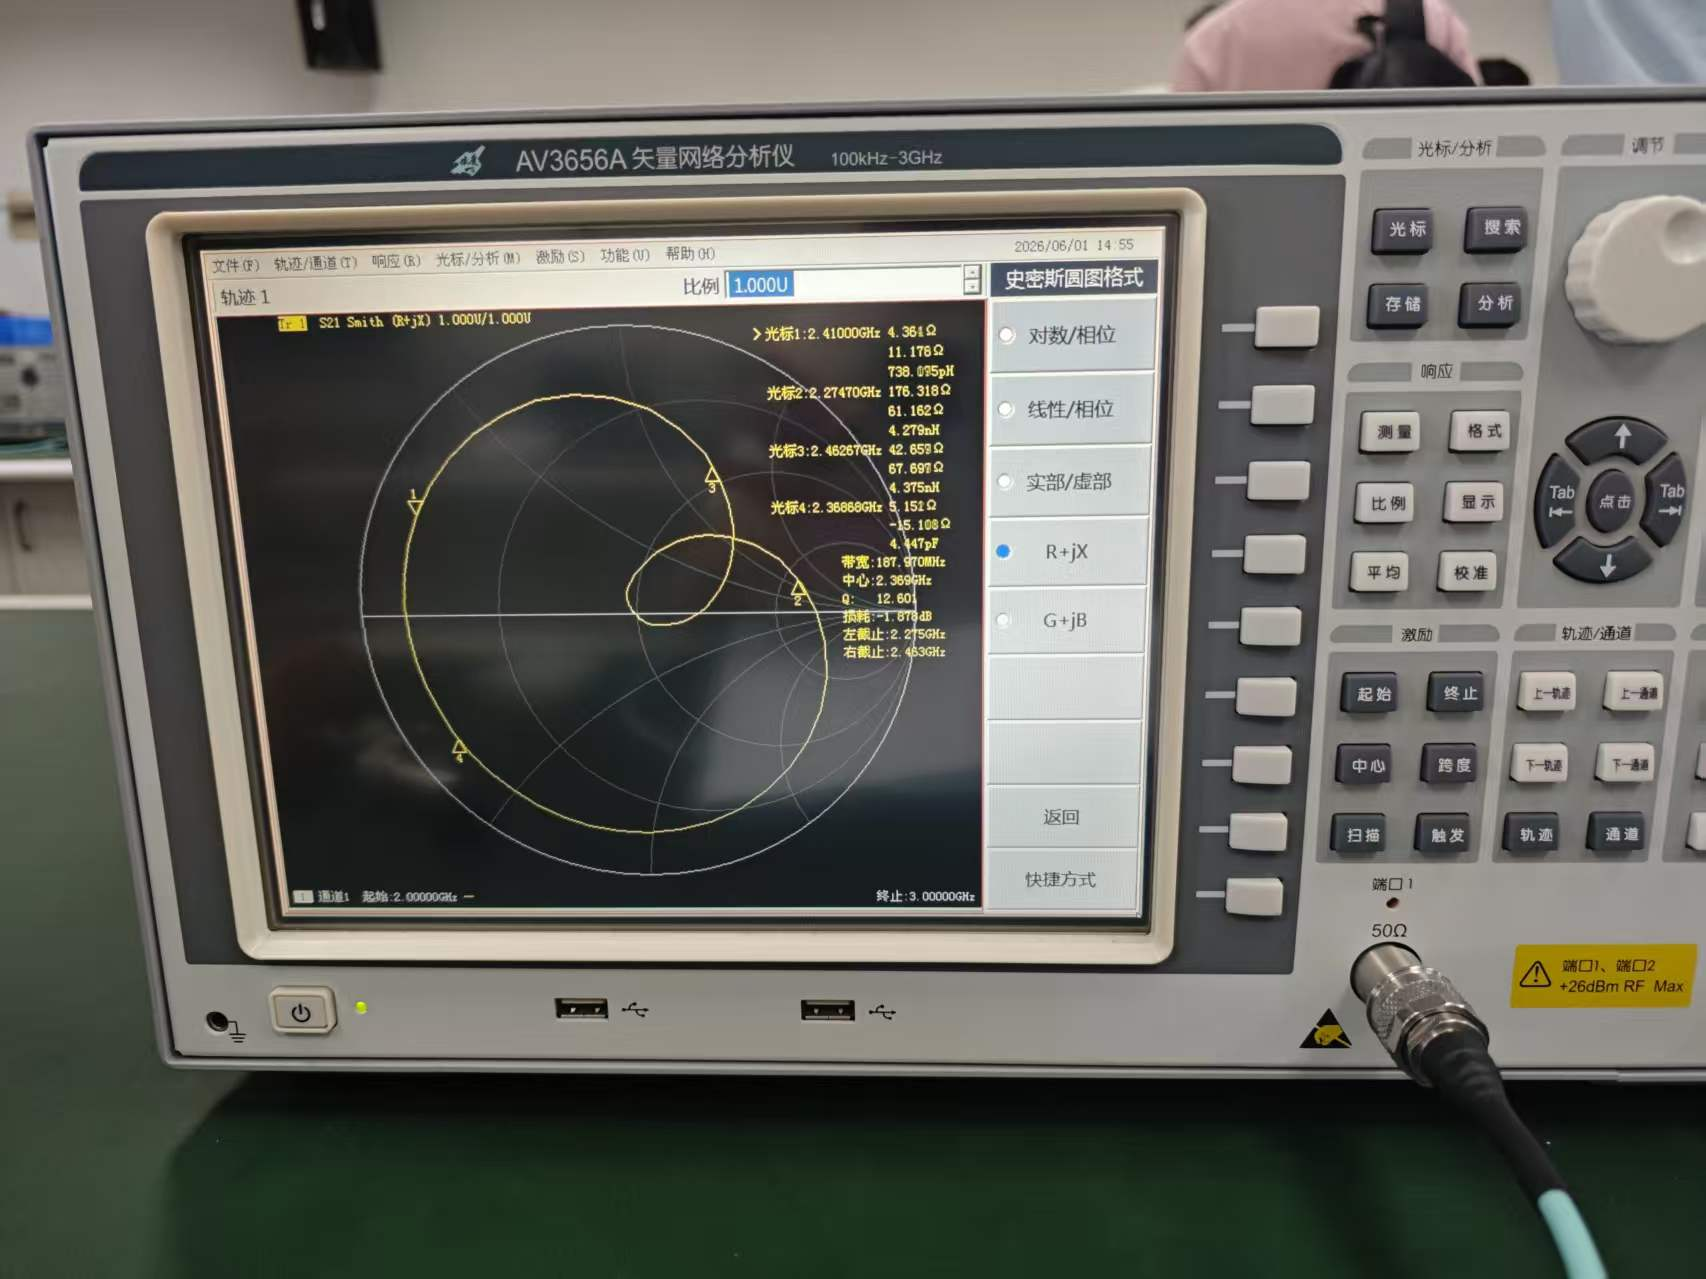
\includegraphics[width=\textwidth]{figures/interference_smith_ref.png}
    \caption{S21 Smith 显示：扰动前}
  \end{subfigure}
  \hfill
  \begin{subfigure}[b]{0.45\textwidth}
    \centering
    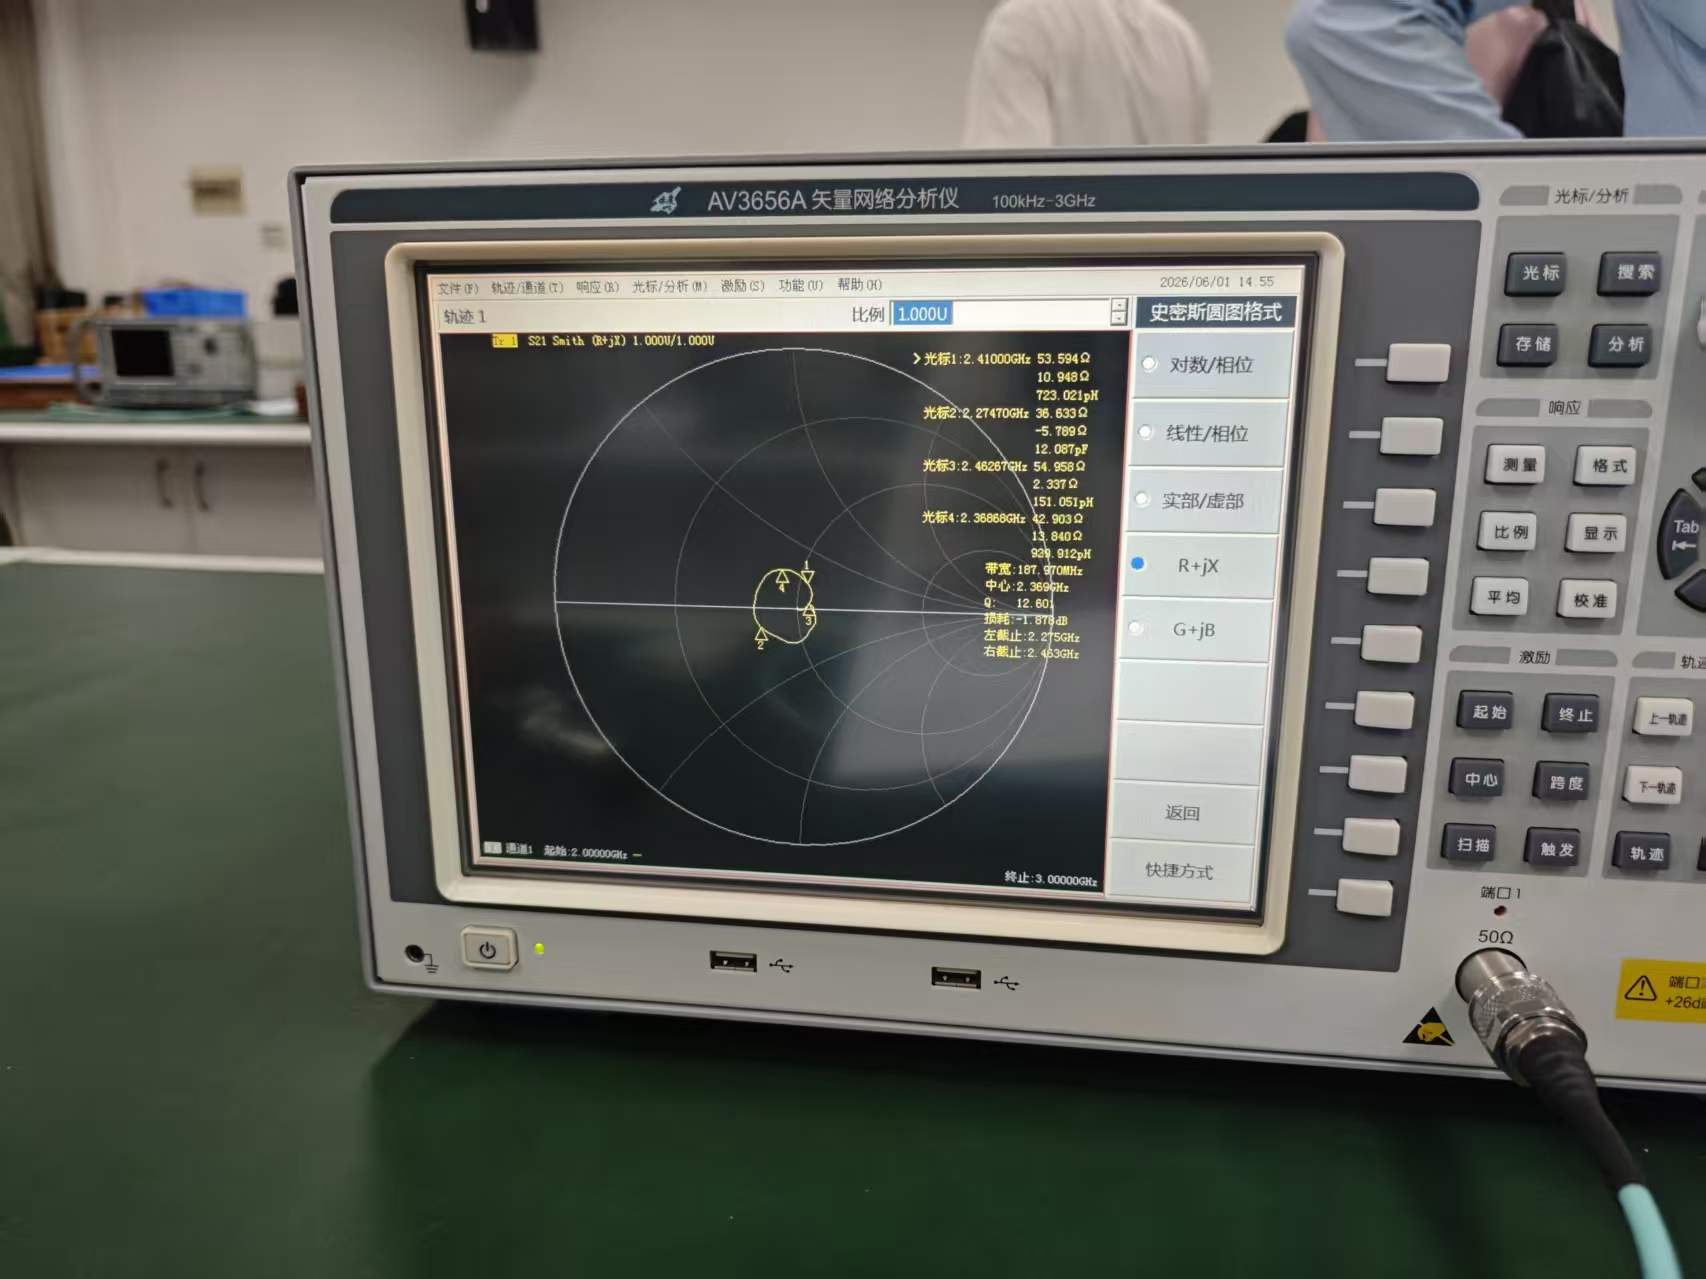
\includegraphics[width=\textwidth]{figures/interference_smith_disturbed.png}
    \caption{S21 Smith 显示：扰动后}
  \end{subfigure}
  \vspace{0.4em}
  \begin{subfigure}[b]{0.45\textwidth}
    \centering
    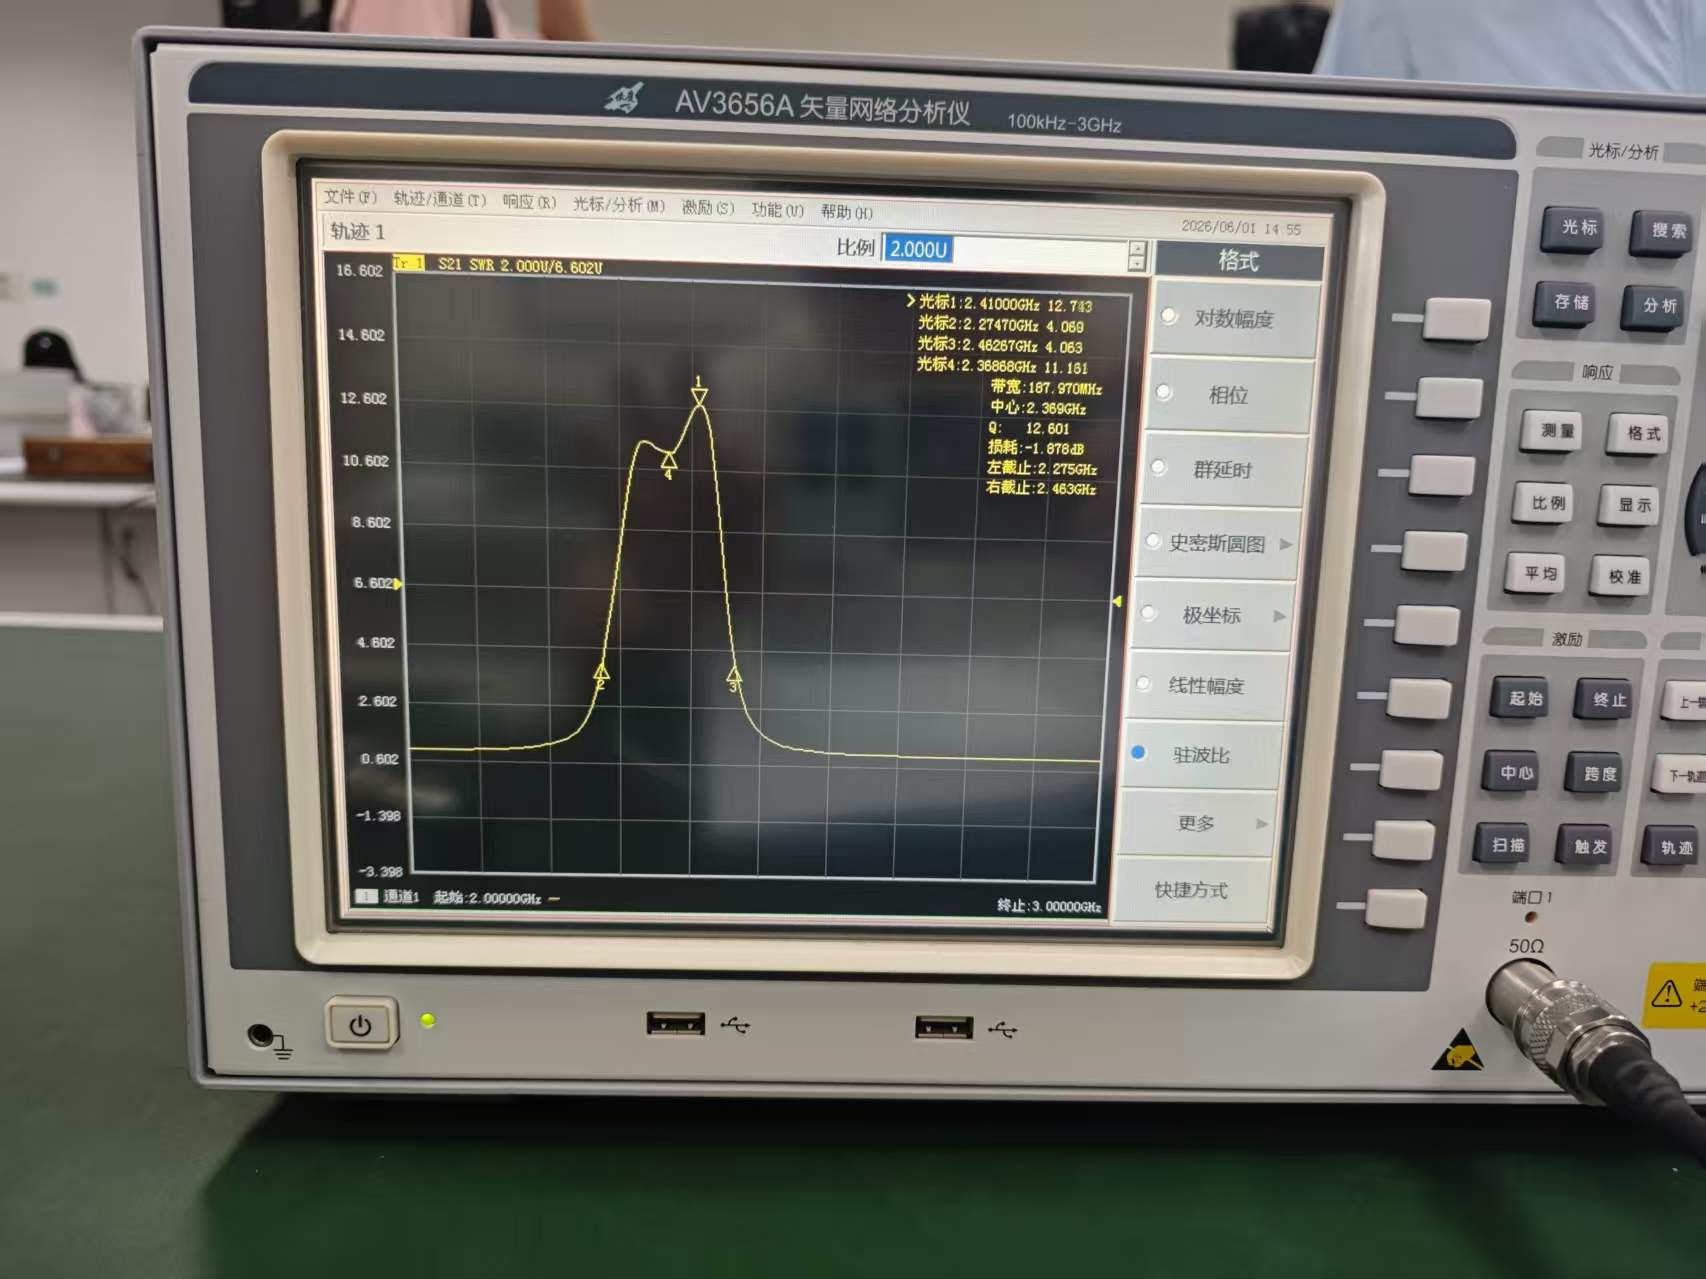
\includegraphics[width=\textwidth]{figures/interference_vswr_ref.png}
    \caption{S21 驻波比显示：扰动前}
  \end{subfigure}
  \hfill
  \begin{subfigure}[b]{0.45\textwidth}
    \centering
    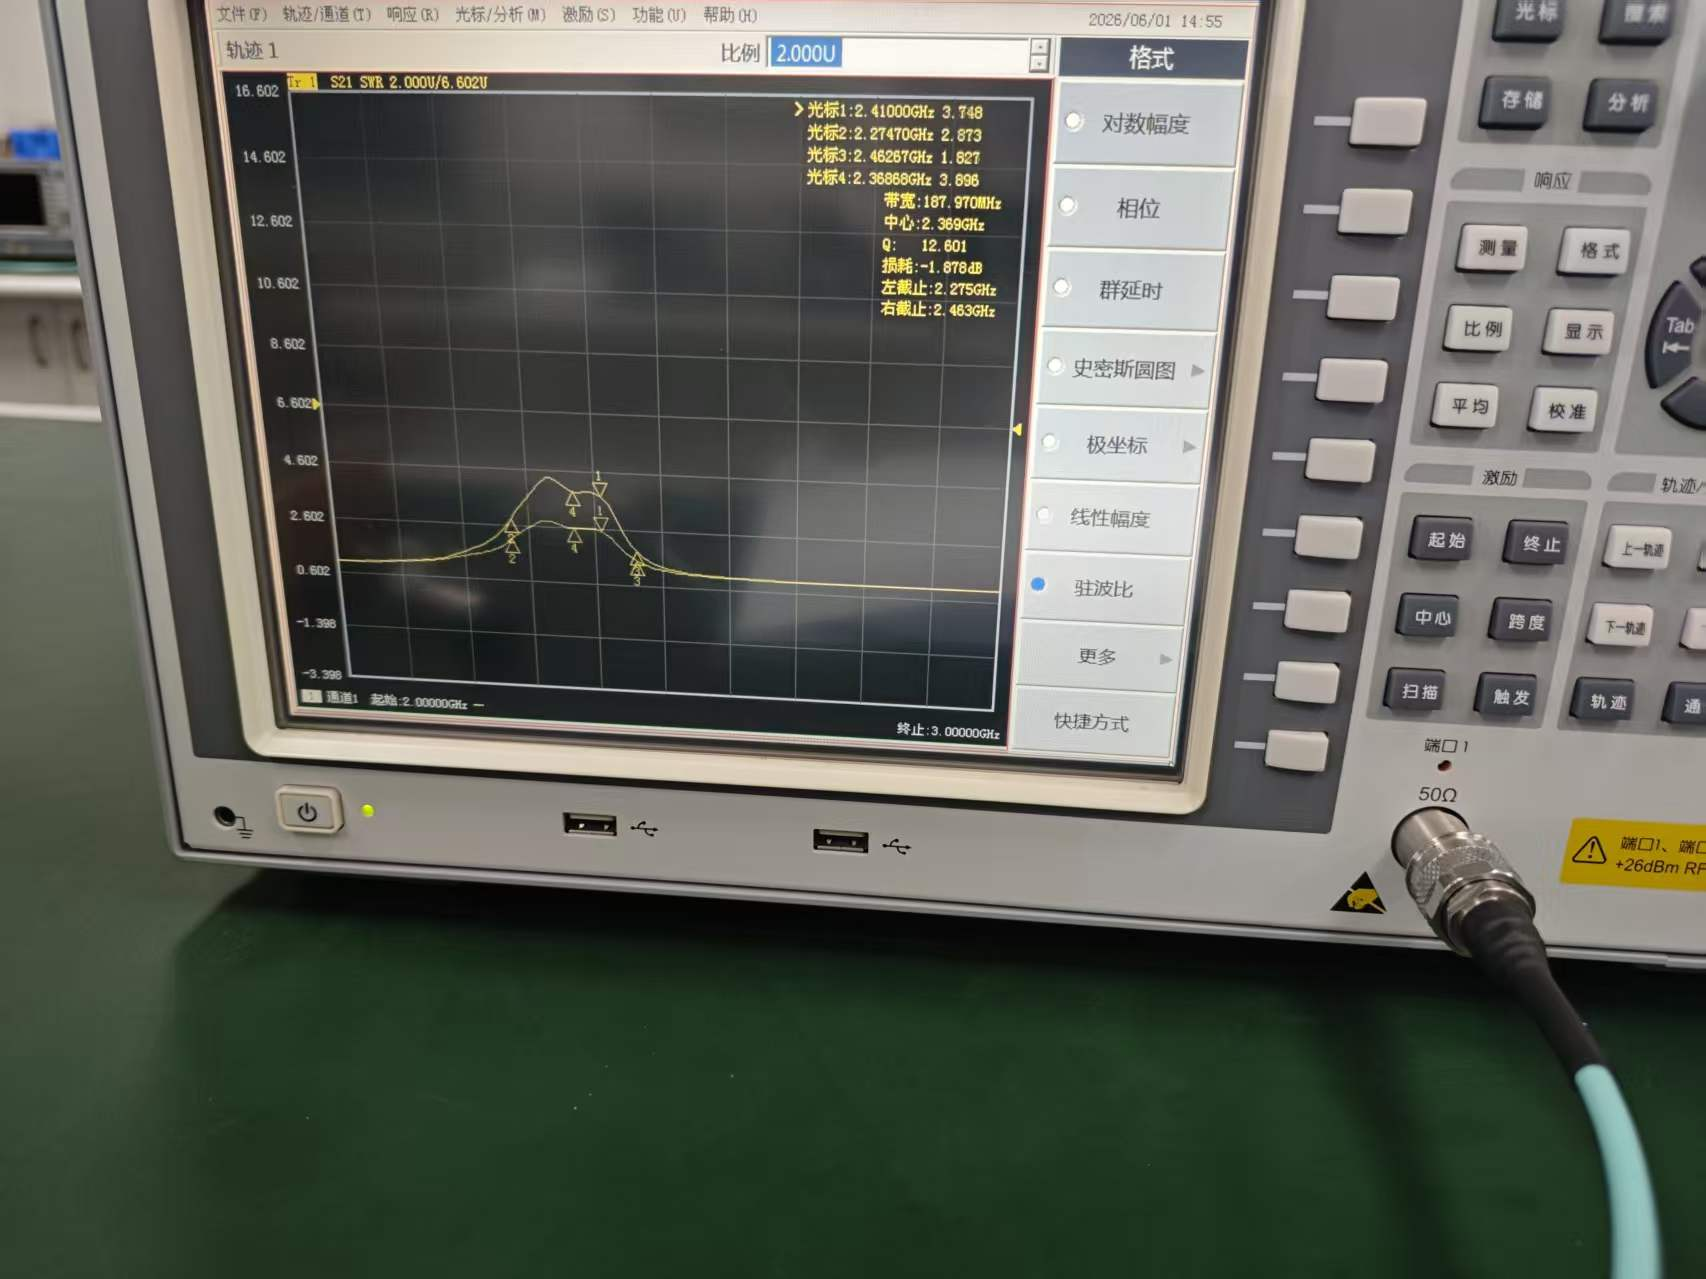
\includegraphics[width=\textwidth]{figures/interference_vswr_disturbed.png}
    \caption{S21 驻波比显示：扰动后}
  \end{subfigure}
  \caption{外界扰动对 S21 Smith 轨迹与驻波比显示的定性影响}
  \label{fig:interference-qualitative}
\end{figure}

图 \ref{fig:interference-qualitative} 中的 Smith 圆图和驻波比是在 S21 传输测量状态下得到的，不能按 S11 的方式直接定量解释为输入阻抗或端口驻波比。若需得到滤波器输入阻抗，应切换到 S11 并进行相应校准。这里可作定性观察：扰动后 S21 的 Smith 轨迹位置和形状发生改变，驻波比显示中的峰值高度、宽度也随之变化，与对数幅度图中通带衰减增大的现象一致，说明外界扰动改变了滤波器的耦合和损耗状态。

\section{误差来源与讨论}

\subsection{校准与参考面误差}

单端口校准把参考面移动到射频电缆末端，但微带模块仍需经过 N-SMA 转接头、SMA 座和微带过渡结构。这些部件的相位延迟和阻抗不连续不能完全由校准消除，会使 Smith 圆图轨迹旋转或偏离中心。二端口测量中，直通校准状态与滤波器实测连接状态若存在细微差别，也会引入传输幅度和相位误差。

\subsection{端接接触与寄生参数}

贴片元件通过镊子压接到微带端部，接触压力、焊盘位置和元件姿态都会改变串联接触电阻、寄生电感和寄生电容。1 pF 与 3.3 nH 这类小值元件在 2.5 GHz 附近的电抗只有几十欧姆量级，少量寄生参数就会明显改变端口等效值。因此表 \ref{tab:cap-load} 和表 \ref{tab:ind-load} 中的等效量更适合作为被测结构整体响应，不宜简单理解为贴片元件的低频标称值。

\subsection{仪器显示与读数误差}

矢网光标读数受频率步进、显示格式、光标位置和有效位数影响。天线 S11 使用对数幅度显示，数据处理中需先换算为线性 $|\Gamma|$ 再与驻波比对应；滤波器相位显示存在 $\pm180^\circ$ 包裹，分析时应关注相位随频率的连续变化趋势，而不是把显示跳变理解为物理突变。

\subsection{外界环境影响}

微带线与滤波器有一部分电磁场分布在空气中，手指、金属片、仪器外壳、电缆弯折和桌面附近物体都会改变边界条件。外界干扰测试中，S21 通带附近下降超过 20 dB，说明开放式微带结构对环境高度敏感。测量时保持电缆形态、连接器受力和周围物体位置稳定，是提高重复性的关键。

\section{思考题}

\subsection{简述 S 参数的定义及物理意义，说明 S11、S21 的含义}

S 参数用端口入射波和出射波的比值描述线性微波网络。对于二端口网络，有 $b_1=S_{11}a_1+S_{12}a_2$、$b_2=S_{21}a_1+S_{22}a_2$。$S_{11}$ 是端口 1 的反射系数，反映端口匹配程度；$S_{21}$ 是端口 1 到端口 2 的正向传输系数，反映信号通过被测网络后的幅度衰减和相位变化。对负载和天线，S11 可换算输入阻抗、反射系数和驻波比；对滤波器，S21 可确定通带、阻带、插入损耗、中心频率和带宽。

\subsection{若不进行校准，直接接入射频电缆和电路模块测量，会对结果产生什么影响？请分析原因}

若不校准，仪器测到的是仪器端口、电缆、转接头、连接器和被测件的总响应。电缆损耗会改变幅度，电缆长度会引入频率相关相位，连接器不连续会产生附加反射，仪器方向性和源匹配误差也会叠加到结果中。表现到 Smith 圆图上，轨迹会整体旋转、缩放或偏移；表现到 S21 上，插入损耗和相位斜率不再只属于被测滤波器。因此矢网测量必须先通过校准确定参考面。

\subsection{设计实验方案，测量 N-SMA 转接头对测试曲线的影响}

可采用反射和传输两种对比方法。反射测量中，先在射频电缆 N 端完成单端口校准，接入 N-SMA 转接头和已知 SMA 匹配负载测量 S11；再用 N 型匹配负载直接测量 S11，两条曲线的差异可反映转接头引入的附加反射和相位变化。传输测量中，完成二端口直通校准后插入一对背靠背 N-SMA/SMA-N 转接头，测量其 S21 幅度和相位；若仪器支持端口延伸或时域功能，还可进一步估算转接头等效电长度和局部不连续位置。

\subsection{根据实验给出的微带线设计参数，计算 50 $\Omega$ 半波长微带线的宽度和长度}

忽略铜厚修正时，对于 $W/h>1$ 的微带线有
\begin{equation}
  \Zzero=\frac{120\pi}
  {\sqrt{\varepsilon_\mathrm{eff}}\left(W/h+1.393+0.667\ln(W/h+1.444)\right)},
\end{equation}
\begin{equation}
  \varepsilon_\mathrm{eff}=
  \frac{\varepsilon_r+1}{2}+
  \frac{\varepsilon_r-1}{2}\left(1+\frac{12h}{W}\right)^{-1/2}.
\end{equation}
代入 $\varepsilon_r=4.6$、$h=0.765\,\mathrm{mm}$ 并令 $\Zzero=50\,\Omega$，数值求解得
\[
  W/h\approx1.86,\quad W\approx1.43\,\mathrm{mm},\quad
  \varepsilon_\mathrm{eff}\approx3.46.
\]
在 $f_0=2.5\,\mathrm{GHz}$ 时，
\[
  \lambda_g=\frac{c}{f_0\sqrt{\varepsilon_\mathrm{eff}}}\approx64.47\,\mathrm{mm},
\]
因此半波长微带线长度约为
\[
  l=\frac{\lambda_g}{2}\approx32.23\,\mathrm{mm}.
\]
实际加工时还需考虑开路端延伸、焊盘、转接头和介质参数偏差，故计算结果主要作为设计初值。

\section{实验收获与建议}

\subsection{实验收获}

通过本次测量，可以直观理解微波频段中“负载值”和“端口看到的等效阻抗”之间的区别。49.9 $\Omega$ 电阻在低频电路中几乎可以看作理想匹配负载，但接入微带结构后，转接头、传输线电长度和压接位置会带来可观察的虚部；开路、短路、电容和电感负载则在 Smith 圆图上表现出不同方向的轨迹旋转。由这些现象可以看出，传输线理论并不是孤立公式，而是直接决定矢网屏幕上曲线形态的物理原因。

滤波器和天线测量进一步加深了对 S 参数用途的理解。S21 幅度曲线能够直接给出滤波器的通带、插入损耗和带宽，相位曲线体现信号通过网络后的相移；S11 与驻波比则适合评价天线匹配程度。外界干扰测试说明开放式微带结构对周围环境十分敏感，也让校准参考面、连接稳定性和测试条件一致性的重要性更加明确。

\subsection{实验建议}

实验记录可按“测量对象、校准方式、端口设置、显示格式、频点读数、环境条件”建立统一表格。这样在整理数据时，S11、S21、Smith 圆图、对数幅度和驻波比之间的对应关系更清楚，也能避免不同显示格式下的数据混用。对于贴片负载，可使用更稳定的夹具或固定压接位置，减小手持镊子带来的接触变化。

滤波器外界干扰测试可进一步设置可重复的扰动条件，例如固定金属片距离、固定覆盖面积或固定手指靠近位置，并分别记录 S21 幅度、中心频率和带宽变化。若条件允许，还可把实测结果与电磁仿真曲线对比，从而区分加工偏差、介质参数偏差和测量环境对结果的影响。

\section{结论}

实验完成了微带传输线负载反射特性、微带耦合滤波器传输特性和天线驻波比的矢网测量。49.9 $\Omega$ 电阻负载的 Smith 圆图轨迹最接近中心，2.7 GHz 处 $|\Gamma|\approx0.057$、VSWR $\approx1.12$；开路、短路、1 pF 电容和 3.3 nH 电感负载均表现出较强反射，并呈现出符合传输线变换规律的感性或容性特征。滤波器实测中心频率约 2.369 GHz，3 dB 带宽约 187.970 MHz，插入损耗约 1.878 dB，具有明确带通响应；外界扰动可使原通带 S21 下降 20 dB 量级，说明开放式微带滤波器对环境变化敏感。天线在 1.65 GHz 附近匹配最佳，2.47 GHz 附近驻波比约 2.25，匹配效果一般。整体结果与传输线反射、Smith 圆图和微波网络参数理论相一致。

\end{document}
